%% This is file `elsarticle-template-5-harv.tex',
%%
%% Copyright 2009 Elsevier Ltd
%%
%% This file is part of the 'Elsarticle Bundle'.
%% ---------------------------------------------
%%
%% It may be distributed under the conditions of the LaTeX Project Public
%% License, either version 1.2 of this license or (at your option) any
%% later version.  The latest version of this license is in
%%    http://www.latex-project.org/lppl.txt
%% and version 1.2 or later is part of all distributions of LaTeX
%% version 1999/12/01 or later.
%%
%% The list of all files belonging to the 'Elsarticle Bundle' is
%% given in the file `manifest.txt'.
%%
%% Template article for Elsevier's document class `elsarticle'
%% with harvard style bibliographic references
%%
%% $Id: elsarticle-template-5-harv.tex 159 2009-10-08 06:08:33Z rishi $
%% $URL: http://lenova.river-valley.com/svn/elsbst/trunk/elsarticle-template-5-harv.tex $
%%
\documentclass[preprint,authoryear,12pt]{elsarticle}
%% Use the option review to obtain double line spacing
%% \documentclass[authoryear,preprint,review,12pt]{elsarticle}

%% Use the options 1p,twocolumn; 3p; 3p,twocolumn; 5p; or 5p,twocolumn
%% for a journal layout:
%% \documentclass[final,authoryear,1p,times]{elsarticle}
%% \documentclass[final,authoryear,1p,times,twocolumn]{elsarticle}
%% \documentclass[final,authoryear,3p,times]{elsarticle}
%% \documentclass[final,authoryear,3p,times,twocolumn]{elsarticle}
%% \documentclass[final,authoryear,5p,times]{elsarticle}
%% \documentclass[final,authoryear,5p,times,twocolumn]{elsarticle}

%% if you use PostScript figures in your article
%% use the graphics package for simple commands
%% \usepackage{graphics}
%% or use the graphicx package for more complicated commands
%% \usepackage{graphicx}
%% or use the epsfig package if you prefer to use the old commands
%% \usepackage{epsfig}

%% The amssymb package provides various useful mathematical symbols
\usepackage{amssymb}
\usepackage{amsmath}
%% The amsthm package provides extended theorem environments
%% \usepackage{amsthm}
\usepackage{color}
\usepackage{soul}  % Remove on submission
\usepackage{siunitx}
\usepackage{array}
\usepackage{lineno}
\usepackage[utf8]{inputenc}
\newcommand{\rpm}{\raisebox{.2ex}{$\scriptstyle\pm$}}
\inputencoding{utf8}
%% The lineno packages adds line numbers. Start line numbering with
%% \begin{linenumbers}, end it with \end{linenumbers}. Or switch it on
%% for the whole article with \linenumbers after \end{frontmatter}.
%% \usepackage{lineno}

%% natbib.sty is loaded by default. However, natbib options can be
%% provided with \biboptions{...} command. Following options are
%% valid:

%%   round  -  round parentheses are used (default)
%%   square -  square brackets are used   [option]
%%   curly  -  curly braces are used      {option}
%%   angle  -  angle brackets are used    <option>
%%   semicolon  -  multiple citations separated by semi-colon (default)
%%   colon  - same as semicolon, an earlier confusion
%%   comma  -  separated by comma
%%   authoryear - selects author-year citations (default)
%%   numbers-  selects numerical citations
%%   super  -  numerical citations as superscripts
%%   sort   -  sorts multiple citations according to order in ref. list
%%   sort&compress   -  like sort, but also compresses numerical citations
%%   compress - compresses without sorting
%%   longnamesfirst  -  makes first citation full author list
%%
%% \biboptions{longnamesfirst,comma}

% \biboptions{}

\journal{Biosystems Engineering}

\begin{document}

\begin{frontmatter}

%% Title, authors and addresses

%% use the tnoteref command within \title for footnotes;
%% use the tnotetext command for the associated footnote;
%% use the fnref command within \author or \address for footnotes;
%% use the fntext command for the associated footnote;
%% use the corref command within \author for corresponding author footnotes;
%% use the cortext command for the associated footnote;
%% use the ead command for the email address,
%% and the form \ead[url] for the home page:
%%
%% \title{Title\tnoteref{label1}}
%% \tnotetext[label1]{}
%% \author{Name\corref{cor1}\fnref{label2}}
%% \ead{email address}
%% \ead[url]{home page}
%% \fntext[label2]{}
%% \cortext[cor1]{}
%% \address{Address\fnref{label3}}
%% \fntext[label3]{}

% \title{An Autonomous Platform for Use in Kiwifruit Orchards}
\title{A Modular Platform for Autonomous Navigation in Kiwifruit Orchards}

%% use optional labels to link authors explicitly to addresses:
%% \author[label1,label2]{<author name>}
%% \address[label1]{<address>}
%% \address[label2]{<address>}

% \author{Mark H. Jones, Jamie Bell, Matthew Seabright, Joshua Barnett, Alistair Scarfe, Bruce MacDonald, Mike Duke}

%% Group authors per affiliation:
\author[UoW]{Mark H. Jones\corref{mjemail}}
\cortext[mjemail]{markhedleyjones@gmail.com}

\author[UoA]{Jamie Bell\corref{jbemail}}
\cortext[jbemail]{jamie977@gmail.com}
\author[UoW]{Matthew Seabright}
\author[RPL]{Alistair Scarfe}
\author[UoW]{Mike Duke}
\author[UoA]{Bruce MacDonald}

\address[UoW]{School of Engineering, University of Waikato, Hamilton, New Zealand}
\address[UoA]{Faculty of Engineering, University of Auckland, Auckland, New Zealand}
\address[RPL]{Robotics Plus Ltd, Newnham Innovation Park, Tauranga, New Zealand}


\begin{abstract}
%% Text of abstract
    Horticultural robots designed for in-field use generally require a means of transport around farms or orchards.
    A common approach is to directly integrate a drive system at the expense of increasing overall complexity.
    Alternatively, the robots can be modularised and attached to general purpose platforms.
    General purpose platforms reported previously are designed to carry relatively light payloads orientated toward ground based crops.
    This paper presents a modularised platform capable of carrying modules of up to \SI{1000}{\kilo\gram} under \SI{1.5}{\meter} high pergola style kiwifruit canopies.
    Sensors suitable for autonomous navigation are evaluated in-orchard and tested using a prototype navigation algorithm.
    It is found that GNSS based navigation is not feasible under kiwifruit canopies, but perception based navigation sees the platform complete a number of block traversals unassisted.
    The design of the vehicle's structure, drive system, and software architecture is discussed.

    % It is shown that some perception based sensors are suitable for nav
    % It is shown that some perception based navigation sensors are suitable, but GNSS based systems
    % environment due to a lack of GNSS signal reception under canopy.

    % It is shown that GNSS based navigation is inadaquate, but perception based systems

    % It is found that GNSS based systems are not suitable as navigation sensors in this environment

    % % This paper presents a low-slung platform capable of carrying a \SI{1000}{\kilo\gram} payload through GNSS-denied environments, autonomously.
    % The platform is general in the sense that it itself does not perform tasks.
    % It is intended solely to navigate through pergola style orchards while being capable of carrying and supplying power to mounted modules.
    % Navigation sensor selection with in-orchard validation tests are presented.




    % \color{red}Mention that the vehicle operates in a GPS-denied environment\color{black}.
    % Systems for performing autonomous horticultural tasks usually require a means of locomotion through their environment.
    % One approach is to directly integrate a drive system at the expense of increasing overall complexity and development risk.
    % We present a generalised mobile platform designed to carry task specific robots through pergola style kiwifruit orchards.
    % The platform is general in the sense that it itself does not perform tasks.
    % It is intended solely to navigate through orchards and be capable of carrying robotic modules.

    % The selection of sensors best suited for autonomous navigation in this environment is discussed and presented with in-orchard test results.
    % Details of the platform's software and hardware architecture are also discussed.
    % The series-hybrid platform presented here has reliably self-navigated through two test orchards unassisted and is capable of carrying a \SI{1000}{\kilo\gram} payload.
\end{abstract}

\begin{keyword}
%% keywords here, in the form: keyword \sep keyword

%% MSC codes here, in the form: \MSC code \sep code
%% or \MSC[2008] code \sep code (2000 is the default)
    Agricultural automation \sep autonomous navigation \sep orchard robotics
\end{keyword}

\end{frontmatter}

% \linenumbers
% \linenumbers

%% main text
\section{Introduction}
\label{sect:intro}
    Short-term labor requirements within New Zealand's kiwifruit industry peak twice a year corresponding with the pollination and harvesting of kiwifruit.
    The majority of employment during these peaks is filled by seasonal or casual workers \citep{Timmins2009}.
    As kiwifruit is the country's largest horticultural export by value \citep{StatisticsNewZealand2015}, effective automation in this industry will promote economic growth.
    % The New Zealand government aims to double exports from its primary industries between 2012 and 2025 and is actively investing in programmes to achieve this \citep{MinistryPrimaryIndustries2015}.

    Development of an automated kiwifruit harvesting system with integrated drive system has been done before \citep{Scarfe2012}.
    That work presented a platform designed to autonomously navigate though pergola style kiwifruit orchards and had four integrated harvesting arms.
    % The pergola is the most commonly used support structure used to grow kiwifruit in New Zealand.
    Work presented here focuses on creating a platform that operates independently from orchard related tasks, such as fruit harvesting and pollination.
    Utilisation of that base platform will be increased by allowing it to be used during harvesting \emph{and} pollination seasons.
    % This means increasing modularity by separating the task specific systems from the base platform.
    % Harvesting and pollination modules designed for use on the platform have been published elsewhere \citep{williams2017,Seabright2017}.
    Details of modules developed for use on the platform will be published separately.
    These modules have been built as part of a larger project focusing on automation in kiwifruit orchards.

    % Automation in kiwifruit harvesting and pollination demands computer control, state-of-the-art manipulators, and machine-vision based identification systems.
    Automated kiwifruit harvesting and pollination demands computer control, state-of-the-art manipulators, and machine-vision systems.
    Such systems are bulky and have specific geometric requirements dictated by the environment they operate in.
    Both share the need for electrical power, air pressure, and a means of locomotion.
    However, they differ in the way they move when operating.
    The pollinating module moves at a well-known speed with minimum changes in angle.
    This differs from the harvesting module that advances a set distance between stationary harvest cycles.
    To enable the whole system to work autonomously, the base platform must be able to self-drive in a way appropriate for these modules.

    While publishing details of BoniRob, a general purpose robotics platform for field use, the authors stated that ``since the robot development already includes a high complexity, the application itself should be of comparably low complexity'' \citep{Ruckelshausen2009}.
    By separating the development of the platform from other task-specific modules, the risk of a single part becoming overly complex is reduced.
    The presented platform simply needs to navigate through orchards while providing power to modularised systems.

    The development of autonomous vehicles in agriculture is not new, but much of the literature relates to manned vehicles converted to drive-by-wire.
    Because the canopy of a pergola style kiwifruit orchard can droop as low as \SI{1.4}{\meter} to the ground under fruit loading, most standard vehicles are not suited to this environment.
    Many autonomous vehicles designed for use in orchards, such as vineyards, rely on satellite navigation for guidance.
    The dense foliage of a kiwifruit canopy and the surrounding shelterbelts make receiving Global Navigation Satellite System (GNSS) signals unreliable at best.
    This means the vehicle must navigate through its environment using perception based sensors.
    % This paper presents a modularised platform built specifically for use in pergola style orchards.
    % To operate in this environment it must able to:
    Seven requirements have been identified for the platform's use with the pollination and harvesting modules in kiwfiruit orchards.
    These are to:
    \begin{enumerate}
        \item support a mass of \SI{1000}{\kilo\gram},
        \item fit under a \SI{1.4}{\meter} high ceiling,
        \item provide \SI{8}{\kilo\watt} of electrical power to modules,
        \item turn between rows within the headland areas,
        \item include a bin-lifting mechanism for carrying fruit bins,
        \item reliably self-navigate through a test orchard block, and
        \item provide a module mounting area no more than \SI{400}{\milli\meter} from the ground.
    \end{enumerate}
    \begin{figure}[htb]
        \centering
        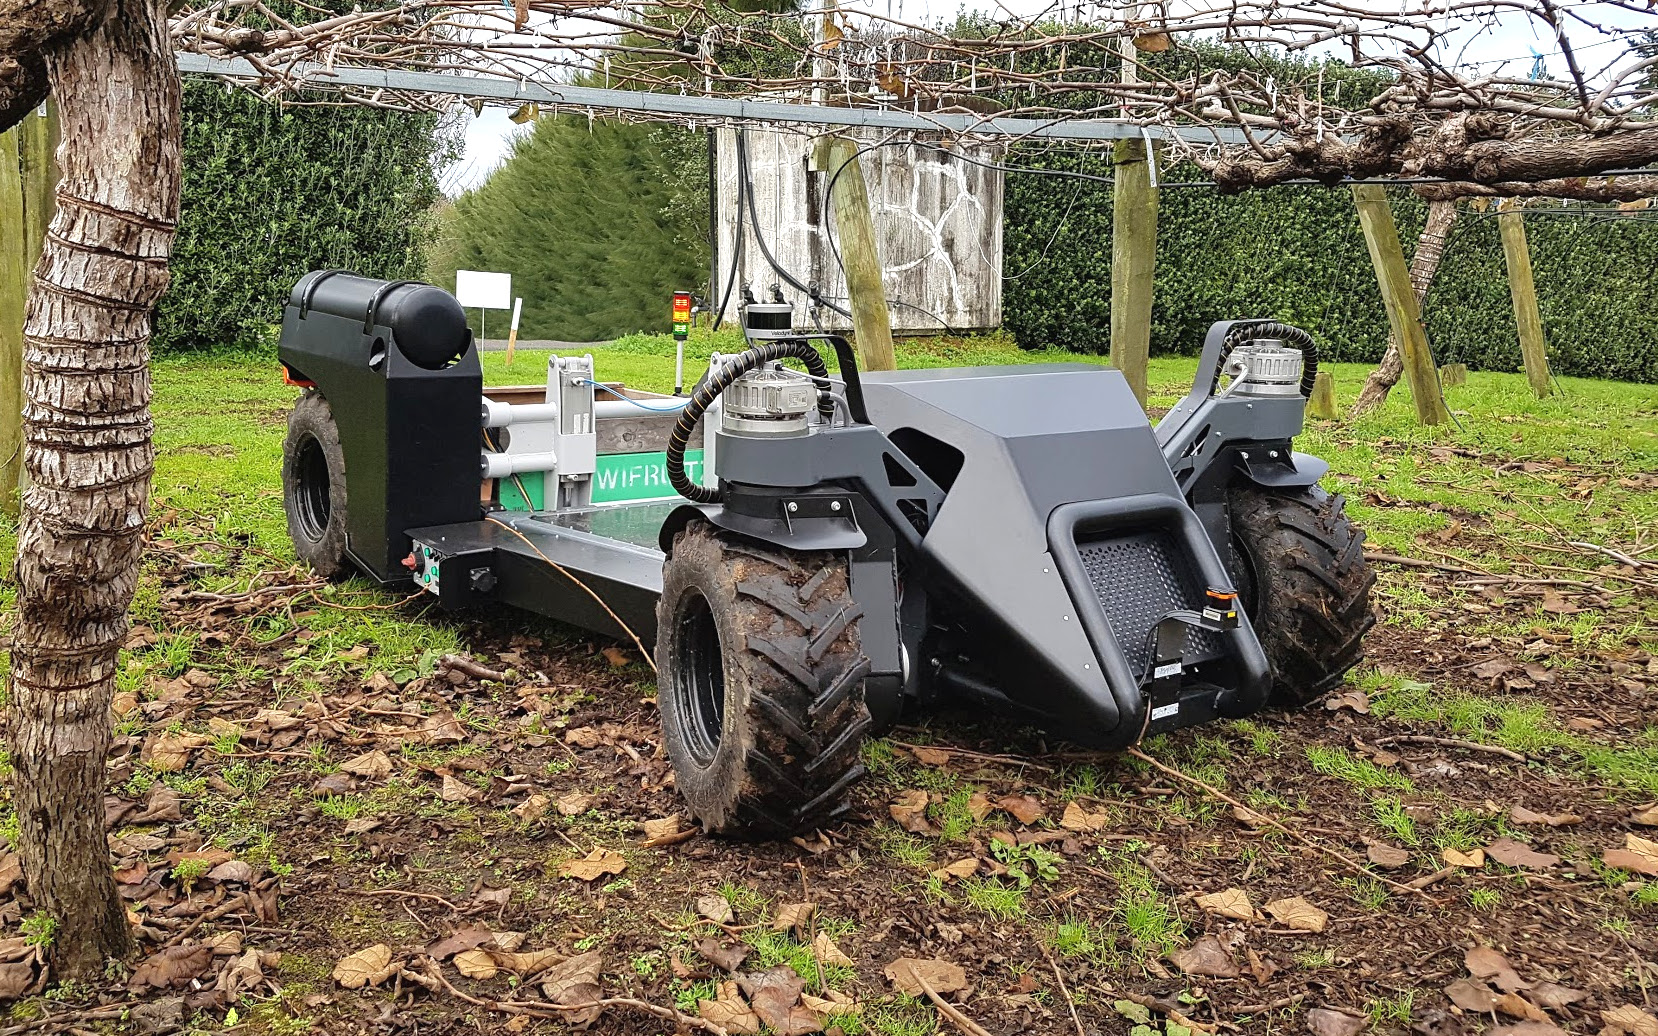
\includegraphics[width=\linewidth]{imgs/photos/suzy_general.jpg}
        % 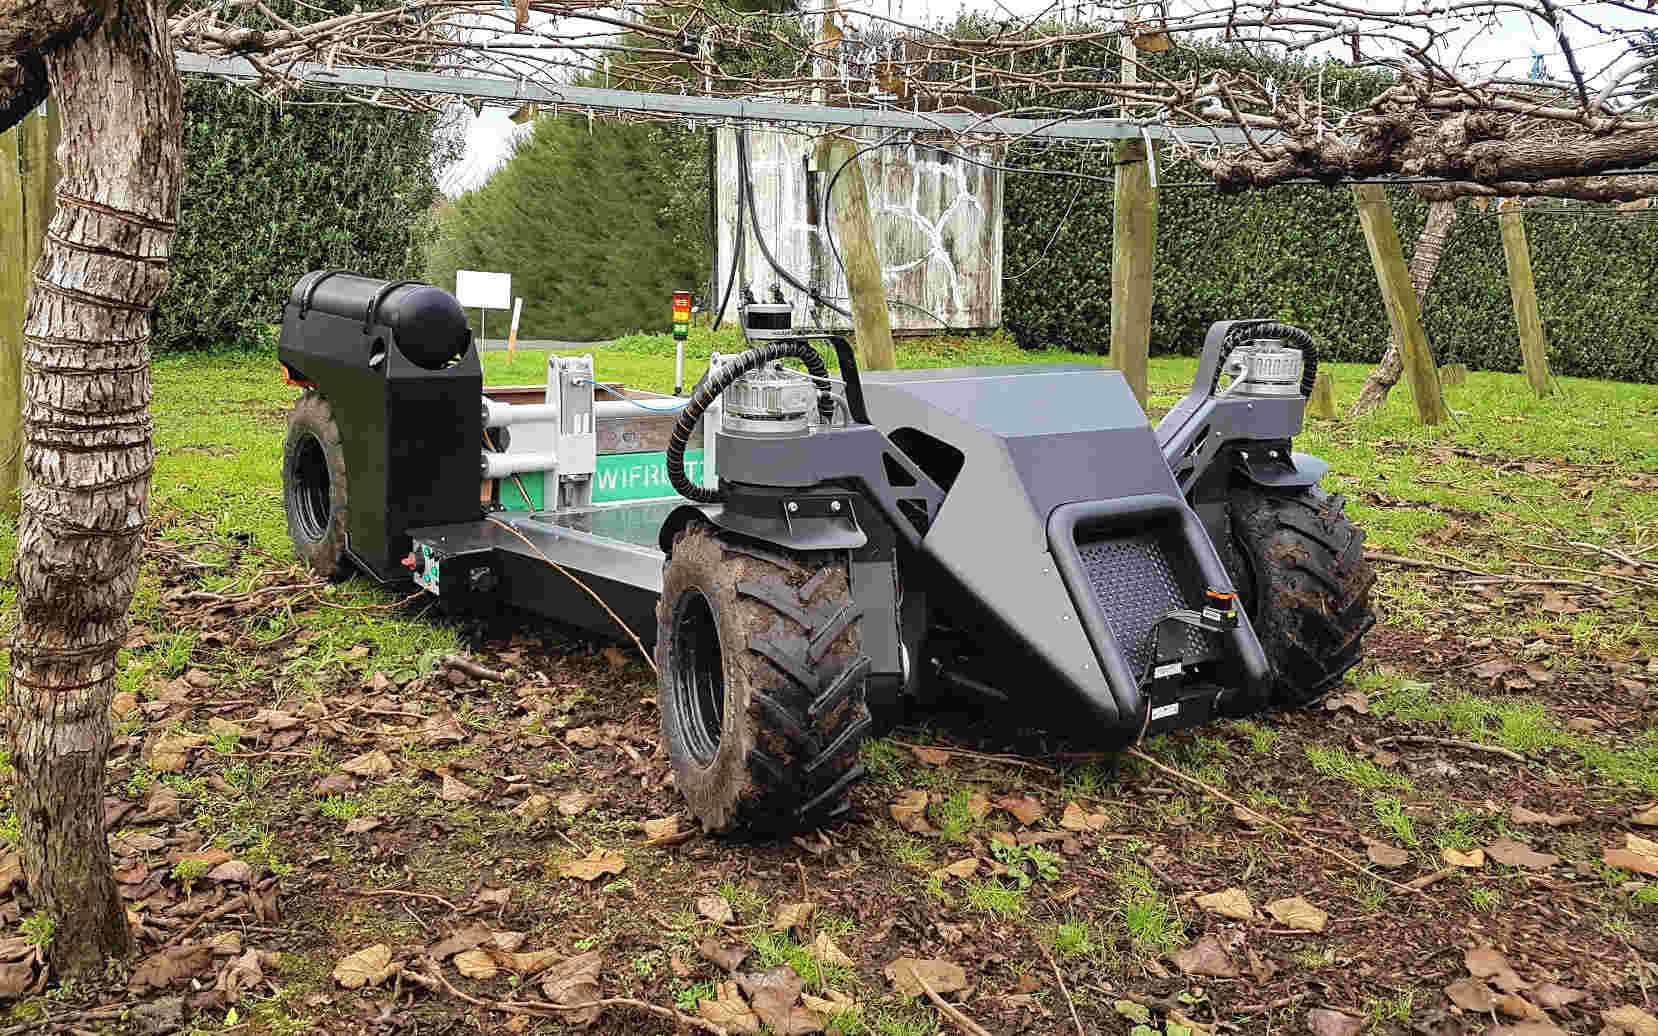
\includegraphics[width=\linewidth]{imgs/photos/suzy_general_small.jpg}
        \caption{
            The platform driving through a row of pergola style kiwifruit orchard while carrying a kiwifruit bin.
        }
        \label{fig:suzy}
    \end{figure}


\section{Related Work}
\label{sect:review}

    \subsection{Purpose-built Autonomous Vehicles in Agriculture}

        The introduction of computers and digital camera technology during the 1980s sparked research into autonomous vehicles for agricultural use \citep{Li2009}.
        When publishing details of an autonomous vehicle in 1998, Tillett et~al.\@ cite difficulties dealing with variability in lighting and the environment as the reason no commercial vehicles were available at the time \citep{Tillett1998}.
        Their vehicle combined wheel encoders, a compass, and accelerometers for odometry information.
        It also featured a camera based row guidance system.
        The system as a whole was capable of spraying individual plants whilst driving autonomously at \SI{0.7}{\meter\per\second} (\SI{2.5}{\kilo\meter\per\hour}).
        % While their purpose built experimental vehicle proved capable of row following and targeted spraying, it was not designed as a modular unit for carrying heavy payloads.
        While their purpose built experimental vehicle proved capable of row following and targeted spraying, it was not designed for modularity.


        % It was capable of spraying individual plants whilst autonomously driving at \SI{0.69}{\meter\per\second} (\SI{2.5}{\kilo\meter\per\hour}).


        Four years later, two autonomous vehicles designed for weed mapping and control in open field crops were presented \citep{Pedersen2002,Astrand2002}.
        These platforms had relatively simple chassis and drive systems as they were both at a prototype stage, i.e., neither were designed to carry heavy payloads.
        The first vehicle, presented by Åstrand \& Baerveldt, featured: two-wheel steering, two-wheel drive, a camera based row guidance system, batteries, a combustion engine, and an air compressor.
        While its appearance resembled that of a computer server rack on wheels, it contained most of the components required of a platform for use with modularised fruit harvesting and pollination modules.
        The second unit, described by Pedersen et~al.\@, was four-wheel drive with two-wheel steering and used GPS as its primary navigation sensor.
        It was battery powered only and lacked any sort of row guidance sensor or power generation unit.
        The authors found that row-crop based navigation from GPS alone was not practical and proposed the integration of a row guidance sensor in their next design.
        They also proposed a revised drive system with four wheel steering and a Controller Area Network (CAN) bus for low-level system communication as opposed to using serial links.


        % Both featured two-wheel steering and were designed specifically for field crops.
        % While both were battery powered, the platform presented by \cite{Astrand2002} could also be fitted with a combustion engine.
        % The vehicle presented by \cite{Pedersen2002} was designed to follow pre-defined GPS based paths through row crops, but the authors found that this was impractical without a dedicated row guidance sensor.
        % They proposed a revised design that featured a row guidance sensor, a revised drive system with four-wheel steering, and a Controller Area Network (CAN) bus for low-level communication.

        Two years later, the revised design proposed by \cite{Pedersen2002} was presented by \cite{Bak2004}.
        % The revised design proposed by \cite{Pedersen2002} was presented two years later by \cite{Bak2004}.
        Its drive system was modularised with four identical drive/steering modules mounted to the chassis for locomotion.
        This revised chassis featured a three-point suspension system that ensured all four wheels stayed in contact with the ground.
        % The GPS receiver on this platform utilised Real Time Kinematic (RTK) corrections from a base station.
        % The use of a fibe-optic gyro, compass, and wheel encoders meant that accurate localisation was still possible in the event of GPS drop-out.
        The system also incorporated the row guidance sensor as proposed in earlier work, as well as a Real-Time Kinematic enabled GPS receiver (RTK-GPS), fiber-optic gyro, compass, and wheel encoders.
        The authors noted that the control strategy for the four independently controlled wheels was non-trivial.
        While much more developed than the previous work of \cite{Pedersen2002}, the platform was not designed to: carry heavy payloads, operate in the absence of satellite navigation, or power itself beyond its battery capacity.
        % Being designed for row-crops, the chassis sits relatively high from the ground with its payload sensors inspecting the ground below.
        % RTK-GPS is capable of providing positioning with accuracies of \SI{2}{\centi\meter}.


        In 2009, details of BoniRob were published by \cite{Ruckelshausen2009}.
        Similar to the previous unit presented by \cite{Bak2004}, it featured a gyroscope, an RTK-GPS receiver, a CAN bus for communication, and four-wheel steering.
        It introduced the use of both single-plane and multi-layer laser range scanning, known as lidar, for perception and row detection.
        A \SI{2.8}{\kilo\watt} petrol generator could be mounted to the chassis, additional to its on-board batteries.
        It was capable of carrying a \SI{150}{\kilo\gram} payload in its dedicated module space, which happens to be the gross weight of the vehicle presented by \cite{Bak2004}.
        What made BoniRob particularly interesting is its ability to alter its track width by actuating the arms to which its wheels were attached.
        Like the robots before it, BoniRob was designed for use on open field crops.
        During the previous year, some of these authors published details of a much simpler robot named `Weedy' \citep{Klose2008}, also an open field crop based sensing platform.
        BoniRob represents the first of the more general purpose platforms designed to carry modularised payloads.


        Most recently, \cite{Bawden2017} published details of their field crop robot -- Agbot~II.
        For locomotion it uses two driven wheels in a differential drive configuration with castor wheels for support.
        It is battery powered and designed to autonomously return to a shipping container with a built-in solar powered charging station.
        The vehicle is made of two side modules bridged by a modular centrepiece containing instrumentation.
        Side modules contain the drive system, whereas the centrepiece is designed to be specific to the application.
        As with all of the vehicles previously reviewed, its payload carrying capabilities are limited to ground facing modules for inspection, weeding, or spraying of field crops.


        Of particular relevance is the earlier work of Scarfe et~al.\@ on an autonomous kiwifruit picking robot \citep{scarfe2009, Scarfe2012}.
        That work involved the creation of a hydraulically driven platform, with two-wheel steering and four-wheel drive, to which four fruit harvesting arms and a bin lifting mechanism were integrated.
        While that platform was designed to navigate through kiwifruit orchards autonomously, its ability to do so was not tested due to an outbreak of \textit{Pseudomonas syringae pv. actinidiae} (PSA) that closed access to kiwifruit orchards.
        The platform had a petrol engine for on-board power generation and made use of camera and lidar based row guidance sensors.
        It had sufficient carrying capacity, however it lacked the modularity of a general purpose platform, meaning it could only be used to harvest kiwifruit.

        With the exception of the platform presented by \cite{Scarfe2012}, all of the reviewed platforms are designed for open field crops.
        None were designed for harvesting operations and therefore were not capable of carrying bins.
        Referring back to the statement from \cite{Ruckelshausen2009} that ``the application itself should be of comparably low complexity'', one can see why research thus far has focused on simpler tasks such as inspection or weeding.
        However, once designs move past these applications it becomes advantageous to accommodate other shared features.
        % Inclusion of a fork lifting mechanism is a good example of this as its purpose is general enough that most orchard related tasks are benefited by it.
        A fork lifting mechanism is general enough that most orchard related tasks can benefit from it.
        For example, with a harvesting module mounted it can be used to hold a bin in which harvested fruit is collected.
        With a pollination module mounted, it can hold the tank of water used to spray a liquid pollen solution.
        Additionally, the ability to pick up a standard pallet has broad applications in and around orchards.

        \cite{Blackmore2007} envisaged significant reductions in production costs for agricultural robotics by repurposing parts already in use in the agricultural and automotive industry.
        High-power AC motor controllers are one such component which are increasingly being used by automotive manufacturers in electric vehicle offerings.
        Significant cost reductions are possible by using controllers designed for integration by automotive manufacturers as opposed to more general purpose motor controllers.
        While not a physical component, the CAN bus is another example of technology borrowed from the automotive industry.
        Most of the more recent platforms reviewed made use of this communication system for low-level communication.

    \subsection{Sensors for Row Based Navigation in Orchards}

        % Since the platform is designed for autonomy, selecting appropriate sensors and developing the vehicle around these sensors is an important design consideration.
        As the platform is designed for autonomy, selecting appropriate navigation sensors is an important design consideration.
        Sensor combinations for orchard based row detection mostly fall into three categories; camera based, lidar based, or a combination of the two.
        The following section summarises a review of row detection efforts in orchards using these sensors.

        % Lidar come in two flavours: single-plane, and multi-layer.

        \cite{Subramanian2006} tested both camera and lidar (Sick LMS-200) based guidance systems in a citrus fruit orchard.
        Sensors were trialled separately on a tractor retrofitted with a drive-by-wire system.
        Their vehicle was able to navigate a small and simplified path using both machine vision and lidar based approaches at speeds of up to \SI{4.4}{\meter\per\second} (\SI{15}{\kilo\meter\per\hour}).
        They found that lidar proved more accurate until the lidar's data transfer rate became a limiting factor.
        The 2D camera based approach was favorable after this point.
        They suggest that combining the two systems would give more robust guidance as well as providing the ability to detect obstacles.
        No mention of the ability for the image based approach to cope with varying lighting conditions is made.
        These results are promising for use in kiwifruit orchards, where the conditions are similar and where the target operating speed is only \SI{1.39}{\meter\per\second} (\SI{5.0}{\kilo\meter\per\hour}).

        \cite{Barawid2007} demonstrate the use of data from a single-plane lidar (Sick LMS-219) to guide a drive-by-wire tractor through an orchard.
        Their results show real-time processing of lidar data is sufficient to navigate an orchard at \SI{0.36}{\meter\per\second} (\SI{1.3}{\kilo\meter\per\hour}).

        In 2011, two groups published work on the generation of centre lines from camera data taken in orchard rows.
        \cite{He2011} uses traditional machine vision, where \cite{Torres2011} makes use of neural network based image processing.
        Both methods generated valid paths, although He et~al.\@ note that theirs may not be suitable when the environment background becomes complex.
        The neural network based approach of \cite{Torres2011} appeared to cope better with variations in lighting and row spacing.
        Also in 2011, \cite{Hansen2011} showed the use of a single-plane lidar (Sick LMS-200) for vehicle localisation in an orchard.

        The work of \cite{Scarfe2012}, combined traditional camera based image processing techniques with a single-plane lidar (Sick LMS-111).
        The image based approach failed to cope with variability in lighting conditions, however the lidar proved useful for detecting the trunks and posts in kiwifruit orchards.

        \cite{Freitas2012} focused on the detection of people and bins within rows of an apple orchard using lidar (Sick LMS-291), a low-cost inertial measurement unit, and wheel encoders.
        Their algorithm was capable of detecting each obstacle class off-line using data captured from a test orchard.

        \cite{Zhang2014} used a lidar (Hokuyo UTM-30LX) to generate maps of an apple orchard with the aid of artificial landmarks.
        They used an actuated single-plane lidar to generate multi-plane data for use in row and landmark based sensing.
        Placing artificial landmarks in orchards was intended to reduce the effort required to create orchard maps for guidance systems.

        The following year, many of the same authors from  the paper presented by \cite{Zhang2014} write about their autonomous vehicle \citep{Bergerman2015}.
        It describes an electric utility vehicle converted to drive-by-wire with the addition wheel encoders for odometry and a single-plane lidar (Sick LMS-111).
        While not demonstrated detecting obstacles in real-time, their previous work processing offline data \citep{Freitas2012} has potential to be integrated on their platform with the addition of extra computing power.

        Most recently, \cite{Sharifi2015} write about a method to generate centre-lines from 2D images of orchard rows.
        Like the work of \cite{He2011}, the technique offers a way to generate paths from a single camera image without resorting to neural networks.
        However, their future work focuses on increasing robustness to variations in lighting conditions, which indicates issues in this area.
        They state their system has use in being complementary to lidar based navigation.

        % The experiences of \cite{Scarfe2012}, and others, indicate that a lidar outputs data that requires less post-processing to be robust.
        The reviewed work suggests two navigation sensor approaches as being suitable for use in orchards.
        First, the use of lidar saw two of the reported vehicles navigate autonomously through orchard environments, which is encouraging.
        Second, when combining cameras with neural network based processing, robustness to environmental complexities such as light or clutter was improved.
        Reports and previous experience suggest traditional image based processing for navigation failed when the scene became complex or significant variations in lighting occured.

        % Common among these vehicles is the use of sensor fusion, whereby data from multiple sensors is merged and filtered.
        % This provides a way to combine the advantages of multiple sensor types, and the benefit of redundancy  into a single computation space.

        With regards to the use of RTK based GNSS guidance, Slaughter et~al.\@ points out the trade-off of requiring an ``unobstructed `view' of the sky from all parts of the field'' \citep{Slaughter2008}.
        % Additionally, multi-path signal propagation caused by nearby foliage or the geometry of the land itself presents its own mode of failure \citep{Durrant-Whyte2005}.
        % A feasibility analysis by \cite{Pedersen2006} highlighted the use of RTK-GPS systems as a significant cost in yearly subscriptions alone.
        \cite{Durrant-Whyte2005} describe one failure mode of GPS being multipath signal propagation caused by nearby foliage or the geometry of the land itself.
        % This requirement can not be satisfied under the canopy of a kiwifruit orchard which are usually surrounded by tall wind-breaking hedges.
        % \cite{Torii2000} suggests a combination of both RTK-GPS and machine vision systems to be the most promising system going forward based on reductions in costs and increases in performance of these systems.
        % While \cite{Li2009} concludes that either GPS and machine vision, or GPS and lidar will be used together as a development trend.
        \cite{Li2009} conclude that the use of either GPS and machine vision, or GPS and lidar will become a development trend.
        Based on the increased reception requirements, we discount the use of RTK based systems, but still consider the use of general purpose GNSS receivers as a secondary input.

\section{Platform Design}
\label{sect:design}
    % \subsection{Vehicle Configuration}
    % \label{sect:mechanical}

        \begin{figure}[htb]
            \centering
            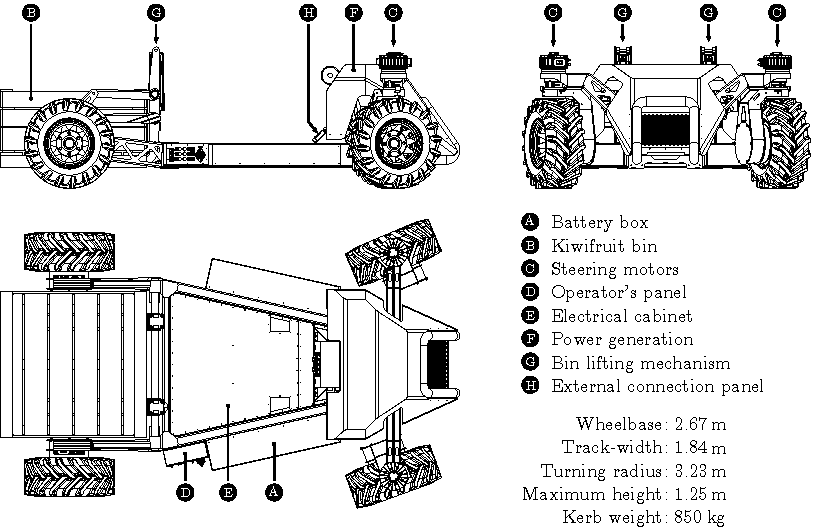
\includegraphics[width=\linewidth]{imgs/profile_views/AMMP-All-Labelled.pdf}
            \caption{Profile drawings of the robotic platform with kiwifruit bin.}
            \label{fig:AMMP}
        \end{figure}

        The vehicle's design is mostly influenced by the need to carry modularised robotic systems and fruit bins.
        Existing commercial platforms suitable for use in horticulture exist, such as the Warthog from ClearPath Robotics, but the maximum payload, battery life, and vehicle geometry make it and similar offerings unsuitable.
        The mass of modules for pollination or harvesting can be as much as \SI{600}{\kilo\gram} and a bin of kiwifruit adds an additional \SI{400}{\kilo\gram}.
        The canopy height in these orchards ranges from \SI{1.4}{\meter} to \SI{1.7}{\meter} so the vehicle must have a low profile.
        Modules carried by the platform require clearance from the canopy in addition to the height they occupy themselves.
        To maximise the space available to these modules the platform must be low-slung at the point they attach.
        Figure \ref{fig:AMMP} illustrates the platform's design, with module area allocated between markers `G' and `H' in the side view (top left).
        The top surface of the chassis in this region sits \SI{360}{\milli\meter} above the ground.

        \begin{figure}[htb]
            \centering
            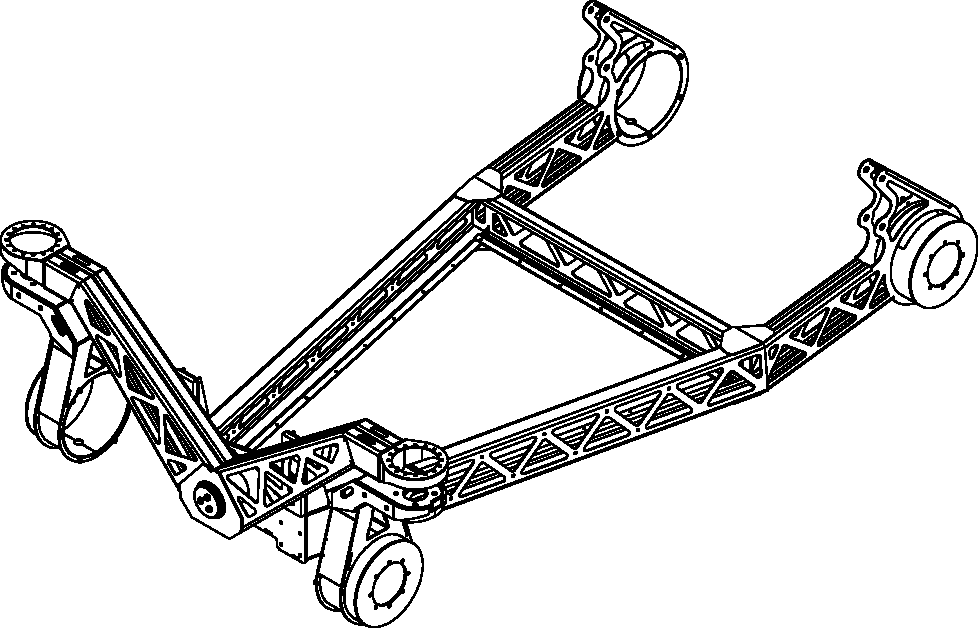
\includegraphics[width=0.6\linewidth]{imgs/profile_views/AMMP-Chassis-1-20.pdf}
            \caption{Drawing of the vehicle's chassis showing front pivot mechanism and steering linkages. The laser-cut and folded structure has a total mass of \SI{190}{\kilo\gram}.}
            \label{fig:AMMPChassis}
        \end{figure}

        The chassis is assembled from sections of \SI{3}{\milli\meter} laser-cut and folded mild steel.
        The sections are welded together on jigs, also made from laser-cut and folded steel, before being powder coated.
        Much of the folded chassis structure contains triangular cut-outs, reducing weight while having minimal impact on rigidity.
        Finite element analysis was used during the design phase to help identify areas needing to be strengthened and areas where material could be removed.
        This helped to ensure the platform meets its target load capacity of \SI{1000}{\kilo\gram}, while the structural chassis weighs only \SI{190}{\kilo\gram}.
        A drawing of the structural chassis is shown as Figure \ref{fig:AMMPChassis}.

        Lifting forks occupy the area between the rear wheels.
        The lifter is actuated by two vertically mounted pneumatic cylinders and is controlled by a standard pneumatic valve block.
        Fuel and compressed air tanks sit over the right-hand rear wheel, while not shown in Figure \ref{fig:AMMP} they can be seen in Figure \ref{fig:suzy}.

    \subsection{Steering}
    \label{sub:steering}

        The angles of the vehicle's front wheels are actuated independently following the Ackermann steering geometry principle.
        Actuation is performed by brushless AC motors (Heinzmann PSM G100) mounted vertically above each drive wheel.
        These motors can generate \SI{7.32}{\newton\meter} of torque with a maximum angular velocity of \SI{3000}{rev\per\minute} and are rated at \SI{2.3}{\kilo\watt}.
        Their outputs are fed through fixed-ratio planetary gearboxes with a 64:1 reduction, increasing torque to \SI{470}{\newton\meter} while reducing the maximum angular velocity to \SI{47}{rev\per\min}.

        % These calculations represent the vehicle loaded with a \SI{1000}{\kilo\gram} mass, sitting on concrete, overcoming the static friction between the tyres and the ground.
        % Torque requirements for the front steering motors were calculated as follows:

        Torque requirements for the steering motors are based on a static friction scenario with the vehicle loaded with a \SI{1000}{\kilo\gram} mass, sitting on concrete.
        This is represented by:
        \begin{equation}
        \label{eqn:steer_torque}
        \tau = W u \sqrt{\frac{B^2}{8} + E^2}
        \end{equation}
        where $\tau$ is the torque required to break static friction, $W$ is the force transmitted through a wheel, $u$ is the coefficient of friction, $B$ is the nominal width of the tyre, and $E$ is the offset between the tyre's contact surface and its axis of rotation.
        The axis of rotation on the vehicle lies directly through the centre of the tyre, meaning $E=0$.
        % As the axis of steering rotation lies directly through the centre of the wheel, $E=0$.
        A value of 0.75 was used as the coefficient of friction as a best guess representation of a tractor-grip tyre on dry concrete.
        The mass of the vehicle (\SI{800}{\kilo\gram}), plus payload (\SI{1000}{\kilo\gram}), and fuel (\SI{60}{\kilo\gram}) adds to \SI{1860}{\kilo\gram}.
        Allowing for uneven weight distribution on the vehicle and a safety margin, the per wheel mass supported is \SI{500}{\kilo\gram}, or a weight of \SI{4900}{\newton}.
        The width of the tyres is \SI{0.28}{\meter}.
        Combining these values in Equation~\ref{eqn:steer_torque} yields a torque of \SI{388}{\newton} to overcome static friction when actuating the steering steering mechanism.

        Actuating the wheels independently removes the need for mechanical linkages between them, allowing for more extreme steering angles and a simpler mechanical design.
        Both steered wheels have the freedom to rotate \SI{330}{\degree}, artificially limited by mechanical stops.
        At the tightest steering angle of \SI{90}{\degree}, the centre-point of the turn is located at the midpoint of the rear wheels.
        The turning radius in this case is roughly equal to the vehicle's wheelbase.
        This sees the vehicle turn between adjacent rows spaced as little as \SI{3}{\meter} apart.
        % It is often possible for the vehicle to make a \SI{180}{\degree} turn mid-row, something not possible for most commercial vehicles designed for orchard use.
        % This range in steering angle allows the vehicle to place the centre of rotation at the mid-point between its rear wheels during its tightest turn.
        % At this steering angle
        Implementing a four-wheel steering system would shift the pivot point to the vehicle's centre, roughly halving the turn radius, but this was deemed unnecessary.

        Headlands in kiwifruit orchards are sized for tractors with much larger turning radii than the developed platform so there is plenty of space for turning.
        Use of a two-wheeled steering system removes the need to develop the ``non-trivial'' control strategies encountered by \cite{Bak2004}.
        It also increases the usable area at the rear of the vehicle by removing the need for clearances around actuated wheels.
        A skid steer system was expected to cause ground damage to a level considered unacceptable to orchard owners when carrying heavy loads.

        The steering motors have incremental encoders, but no means of absolute positioning built-in.
        This means the front wheels angles must aligned before use.
        A homing sequence at boot-up is used to find an absolute angle as a reference for incremental data.
        Inductive proxy sensors are used as a means of detecting the position of the wheels during the homing sequence.

    \subsection{Drive system}
    \label{sub:drive}

        A three point suspension system is used to ensure that all four wheels are in contact with the ground.
        This is achieved with a front pivoting axle, which can be seen in  Figure~\ref{fig:AMMPChassis}.
        As the operating speed for the vehicle is \SI{1.39}{\meter\per\second} (\SI{5.0}{\kilo\meter\per\hour}), the tyres were expected to provide sufficient shock absorption.
        % Shock absorption is provided only by the vehicles tyres
        % The platform has no suspension other than what is provided by its tyres.
        % As the intended operating speed within an orchard is \SI{1.39}{\meter\per\second} (\SI{5}{\kilo\meter\per\hour}), a dedicated suspension system is not considered to be necessary.
        % A three point
        % A front pivoting axle ensures all wheels remain in contact with the ground,  is visible in Figure~\ref{fig:AMMPChassis}.

        % Estimation of the required torque is calculated by the following equations:
        % Calculation of the requirements for the drive system during acceleration up-hill is as follows:

        % Calculation of the drive system's requirements for during up-hill acceleration are as follows:
        Performance requirements for the vehicle's traction system during up-hill acceleration while under load were calculated as follows:
        \begin{align}
        \label{eqn_f_rolling}
        F_{rolling} &= C_{rr} \times m\\
        F_{grade} &= m \times G \times \sin(\alpha)\\
        F_{accel} &= m \frac{\Delta v}{t}\\
        \label{eqn_f_accel}
        F_{total} &= F_{rolling} + F_{grade} + F_{accel}
        \end{align}
        Where $F_{rolling}$ is the force due to rolling resistance; $F_{grade}$ is the a grade, or incline, force; and $F_{accel}$ is the force required for mass acceleration.
        A rolling resistance coefficient ($C_{rr}$) of 0.04 was chosen based on values found in automotive handbooks.
        It represents the case of a pneumatic tyre on medium-hard soil.
        Other variables used are: a vehicle mass ($m$) of \SI{1900}{\kilo\gram}, slope angle ($\alpha$) of \SI{20}{\degree}, velocity change ($\Delta t$) of \SI{2.78}{\metre\per\second} (\SI{10}{\kilo\meter\per\hour}), and an acceleration time ($t$) of \SI{6}{\second}.
        Putting these values through Equations \ref{eqn_f_rolling}--\ref{eqn_f_accel} gives a total force requirement of \SI{7.99}{\kilo\newton}.
        On a per wheel basis this is \SI{2.0}{\kilo\newton}, or \SI{729}{\newton\meter} when taking the wheel radius ($r$) of \SI{0.365}{\meter} into account.
        Required traction power ($P$) is then calculated as follows:
        \begin{align}
        \label{eqn_f_power}
        \omega &= 2 \pi \times \frac{v}{2 \pi r} = \frac{v}{r}\\
        P &= \tau \omega
        \end{align}
        where $\omega$ is the angular velocity of a wheel, $v$ is the vehicle velocity, and $\tau$ is torque.
        At a velocity of \SI{2.78}{\meter\per\second} (\SI{10}{\kilo\meter\per\hour}), the calculations give a power requirement of \SI{5.55}{\kilo\watt} per wheel.

        The selected motors are hub-mounted permanent magnet brushless AC motors with integrated 40:1 fixed-radio planetary gearboxes (Heinzmann PSM-G120).
        Each motor is rated for \SI{6.4}{\kilo\watt} at \SI{96}{\volt} with a maximum angular velocity of \SI{3000}{rev\per\min} and a torque of \SI{20.4}{\newton\meter}.
        At the output of the gearbox, the torque jumps to \SI{816}{\newton\meter} while the angular velocity drops to \SI{75}{rev\per\minute}.
        This gives the platform a top speed of \SI{10.3}{\kilo\meter\per\hour}.

        % Relevant references are \citep{Bosch2002} and \cite{Wong2001}.
        % A rolling resistance coefficient $C_{rr}$ of 0.04 chosen based on values from various automotive handbooks \citep{Bosch2002}.

        In total there are seven brushless AC motors on-board the platform: four drive motors, two steering motors, and a motor used for electrical power generation.
        Each are connected to individual AC motor controllers (Sevcon Gen4 DC Size 4).
        These controllers are available in four bus voltage options: 24-36V, 36-48V, 72V-80V, and 96V-110V.
        The six motors used for traction and steering are together capable of consuming \SI{30.2}{\kilo\watt}.
        With a \SI{48}{\volt}DC bus this would equate to a current draw of \SI{630}{\ampere}.
        As \SI{24}{\meter} of cabling is required to connect the motors and controllers to a common point on the vehicle, a \SI{96}{\volt}DC bus was used to reduce the required gauge of that cable.


    \subsection{Power Distribution}
    \label{sub:power}
        The system bus connects the batteries and generator to motor controllers and on-board power converters.
        A series of heavy-duty contactors (TE Connectivity Kilovac LEV200) control each device's connection to the bus, as well as the bus's connection to the power source.
        Figure \ref{fig:power_system_diagram} illustrates the distribution of power on the platform.

        \begin{figure}[htb]
            \centering
            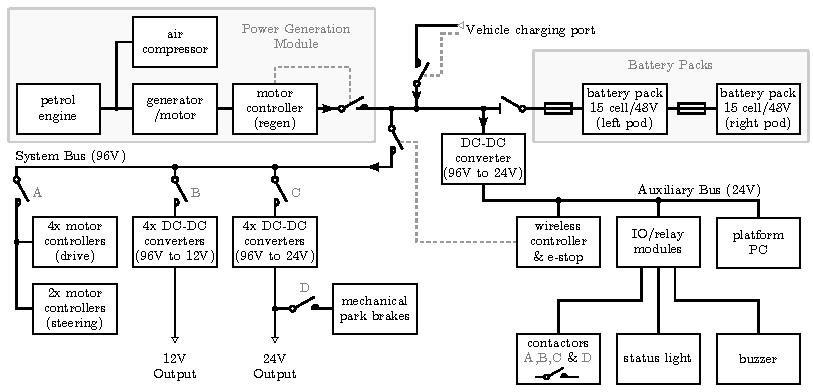
\includegraphics[width=\linewidth]{imgs/system_diagram/full-system-diagram_v1.pdf}
            \caption{Power distribution system diagram. Dashed lines in grey indicate control lines to contactors.}
            \label{fig:power_system_diagram}
        \end{figure}

        Two battery modules attached to the sides of the chassis each house fifteen lithium-iron-phosphate (LiFePO$_{\text{4}}$) batteries connected in series.
        Together, the batteries (Winston/Thundersky WB-LYP90AHA) provide a nominal bus voltage of \SI{96}{\volt} and a total electrical capacity of \SI{8.64}{\kilo\watt\hour}.
        The battery packs were `bottom-balanced' before being fitted and no cell-level voltage monitoring is present.
        Maximum and minimum pack voltages were established by monitoring individual cells during charging and discharging.
        At the point that any individual cell exceeds a safe maximum/minimum threshold, the respective maximum/minimum pack voltage is determined.

        A hermetically sealed disconnect switch (Gigavac HBD41) separates the batteries from the system.
        Once closed, an auxiliary 24V bus becomes powered which powers components required to bring the rest of the rest up.

        A power generation unit comprised of a petrol engine (Honda GX-690), air compressor (Rotorcomp NK-1), and electrical generator is housed at the front of the vehicle.
        The drive shafts of the three units are connected via pulleys and a heavy-duty timing belt.
        The engine, compressor, and alternator are controlled and monitored by a microcontroller based control board.
        This board connects to the Platform PC via the system CAN bus.
        The engine is capable of producing \SI{16}{\kilo\watt}, where up to \SI{9.6}{\kilo\watt} is converted to electrical power, artificially limited in software, and \SI{4.0}{\kilo\watt} is converted to pneumatic power.

        Electrical generation is done with a brushless AC motor/generator (Heinzmann PMSG-150) connected to the same model of motor controller used with the drive system.
        This motor is a larger variant of those used for traction and steering, but with no gearbox fitted.
        Its controller is configured only to have regenerative braking functionality.
        This configuration allows the system to control the power output by adjusting the braking effort required from the controller.
        The controllers offer configuration of battery voltage and current limits as well as the ability to reduce output effort as the battery voltage approaches its maximum.
        These settings provide all the functionality of a general purpose lithium-ion battery charger, making this a cost effective charging solution.
        Electrical energy from the power generation unit is fed to the batteries in a series-hybrid configuration.
        An external charging port is also fitted to allow charging of the batteries without using the petrol engine.

        A fuel tank is fitted over the rear right-hand wheel, visible in Figure~\ref{fig:suzy}.
        It can hold \SI{60}{\litre} of petrol, allowing the vehicle to operate continuously for over \SI{24}{\hour}.
        On-board DC-DC converters deliver \SI{2.8}{\kilo\watt} at \SI{12}{\volt}DC, \SI{3.8}{\kilo\watt} at \SI{24}{\volt}DC, and \SI{3.5}{\kilo\watt} at \SI{240}{\volt}AC, simultaneously.
        A connection panel at the front of the dedicated module area houses the weather-sealed plugs through which these outputs are accessible.


    \subsection{Communications Architecture}
    \label{sect:architecture}

        \begin{figure}[htb]
            \centering
            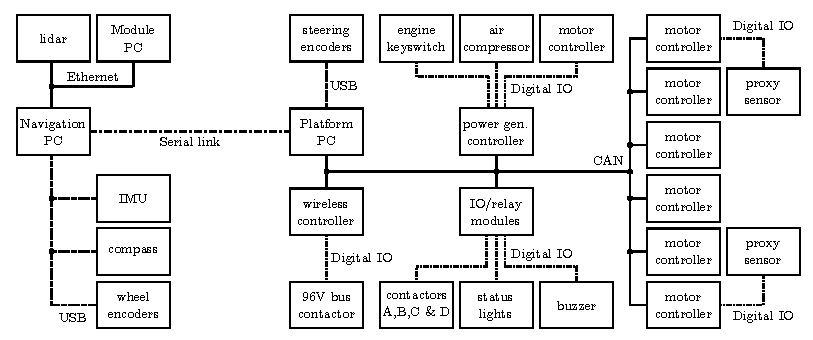
\includegraphics[width=\linewidth]{imgs/system_diagram/diagram_v5.pdf}
            \caption{
                Communications level system diagram showing types of links between devices.
                Devices on right-hand side of the serial link are mechanically integrated into the vehicle, whereas those on the left are modular and can be removed.
            }
            \label{fig:system_diagram}
        \end{figure}

        % This section briefly explains the hardware and software architecture of the platform.
        The platform is centrally controlled by an x86 based small-form-factor PC (Intel NUC) running Ubuntu 16.04 server edition, referred to as the ``Platform PC''.
        This computer communicates with most sub-systems via a CAN bus interfaced using a USB adaptor (IXXAT USB-to-CANV2).

        A second, externally mounted, computer is responsible for higher level control of the vehicle.
        It is used to connect to navigation sensors, send drive commands to the platform, and perform processing tasks relevant to autonomous navigation.
        It too is an x86 based PC running Ubuntu, but uses a commodity microATX form-factor motherboard with a discrete graphics card (Nvidia GTX 1080).
        The graphics card is used to accelerate neural network algorithms and some image processing functions.
        An Ethernet network connects this PC to mounted modules and sensors, whereas a direct serial connection is used to communicate with the Platform PC.
        Figure~\ref{fig:system_diagram} illustrates how these devices are linked together.

        In addition to the drive commands generated by the Navigation PC, a wireless controller (HBC Radiomatic Eco) lets the operator issue drive commands via joystick.
        The receiver module contains relays that are directly controllable from the remote control.
        All inputs from this controller are also broadcast on the CAN bus and read by software nodes on the Platform PC.
        The remote control has two joystick inputs, two selector switches, four buttons, and an emergency stop switch.
        The emergency stop switch is connected to the \SI{96}{\volt} bus contactor via relay outputs from the receiver unit.
        If this switch is closed during operation, or the controller goes out of range, power to the bus is cut within \SI{500}{\milli\second}.
        This engages the mechanical park brakes, removes all tractive effort from the motor controllers, and de-powers mounted modules.

        The open source Robotic Operating System (ROS) is used to facilitate communication between computers and software nodes running within each computer.
        Nodes written using this framework follow either a publish-subscribe or service-client pattern depending on the application.
        % Figure \ref{fig:system_diagram_software} shows a simplified passage of information flowing through the navigation system.
        To maximise code reusability, each device on the platform has its own ROS node dedicated to publishing device data or subscribing to generated device commands.
        Interface adapters, motor controllers, wireless controllers, lidar, and encoders are some devices with dedicated interface nodes.
        Nodes are also used to transform or perform calculations on data while passsing it between nodes written in either C++ or Python.
        For instance, as shown in Figure \ref{fig:system_diagram_software}, an `ackermann kinematics' node transforms steering input data into individual wheel velocity and position/angle outputs.
        Among other things, ROS offers the ability to monitor and record all communication passing through it which can be replayed at a later date.

        A manufacturer's configuration of the motor controllers require them to be interfaced using a combination of analog and digital inputs.
        For example, the accelerator and steering inputs are controlled by potentiometers actuated by the vehicle's driver.
        However, the controllers also provide an option for a multi-motor vehicle configuration.
        In this configuration, inputs fed into a master controller are relayed to a second controller over a CAN interface.
        This interface is configured using a proprietary tool and is not intended for use other than between controllers configured with their software.
        By observing the communication protocol between a master and slave in operation, it was possible to implement a master node in software that runs on the Platform PC.
        With this, all motor controllers on the platform are programmed as slave devices.
        This forces them to accept drive commands via CAN interface, allowing them to be directly controlled by ROS nodes.

        Relay modules allow the Platform PC to toggle power to on-board power supplies, motor controllers, park-brakes, and lights.
        They also monitor the timing of synchronisation messages transmitted by the Platform PC onto the CAN bus.
        These synchronication messages are configured to occur every \SI{20}{\milli\second} as an indication that the system is running as expected.
        Once a relay module detects an absence of these messages for \SI{100}{\milli\second} or longer it enters an error state.
        This causes the motor controllers and on-board power supplies to be shut-off and the park-brakes to be engaged.
        Synchronisation message monitoring is used as a failsafe mechanism to ensure the system is promptly shut-down if the Platform PC fails.

        The open source simulation package Gazebo was used to simulate the vehicle's steering geometry with input from a gamepad.
        This revealed issues that were resolved before implementation on the physical hardware.
        It also provided the opportunity to tune control parameters, such as steering sensitivity, while reducing the time to test.

        \begin{figure}[htb]
            \centering
            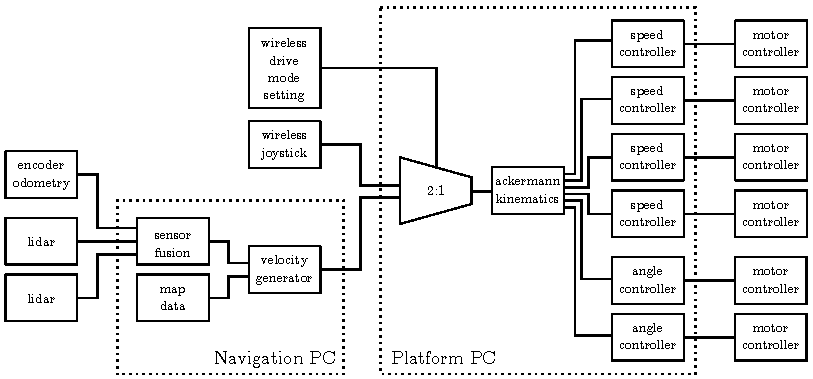
\includegraphics[width=\linewidth]{imgs/system_diagram/software_v2.pdf}
            \caption{Simplified diagram showing connectivity between ROS nodes used for manual and autonomous platform control.
            The `velocity controller' node could implemented using as many as ten or mode separate nodes during development.}
            \label{fig:system_diagram_software}
        \end{figure}

        % Figure \ref{fig:system_diagram} shows a simplified arrangement of connections between each devices.
        % Low-level hardware devices on the platform, such as motor controllers and relays, are connected to the Platform PC via CAN bus.
        % Standardised protocols and software frameworks are employed where possible, supplemented with custom solutions only when needed.


\section{Navigation Sensor Selection}
\label{sect:sensors}
    The choice of sensors incorporated into a vehicle determines which algorithmic approaches are available for navigation and object detection.
    The use of lidar, cameras, and GNSS receivers have been considered.
    Each sensor's ability to capture relevant data is evaluated by in-orchard trials.

    Other sensors considered for inclusion are outlined in Table \ref{table:sensor_comparison} along with their associated issues.
    Factors considered were the strengths and weaknesses in the context of orchard use, reported usage in literature, and availability at a suitable price.
    The review of previous works highlighted both lidar and 2D cameras as offering high functionality for navigation and object detection.
    Time-of-flight cameras are a compelling option based on a cost-benefit analysis; especially if cheaper units work outdoors in the presence of sunlight.
    Because localisation is such a key function, the performance of two GNSS receivers has also been evaluated.

    \begin{table}[htbp]
        \centering
        \footnotesize
        \begin{tabular}{ l l}

            \textbf{Sensor Type}      &\textbf{Common Issues} \\ \hline
            GNSS receiver              & Prone to signal loss from surrounding foliage\\  \hline
            Inertial Measurement Unit & Error accumulation and thermal drift\\ \hline
            Digital Compass           & Prone to disturbance by nearby metallic structures\\ \hline
            Encoder                   & Error accumulation \\ \hline
            Lidar                     & Reduced visibility in fog and heavy rain \\ \hline
            Time of Flight Camera     & Reduced visibility in sunlight, fog and heavy rain \\ \hline
            Camera                    & Reduced visibility in fog or direct sunlight \\ \hline
            Thermal Camera            & Reduced visibility in conditions of low thermal contrast\\ \hline
        \end{tabular}
        \caption{Sensor types considered for inclusion on the platform.}
        \label{table:sensor_comparison}
    \end{table}

    As the drive motors have built-in wheel encoders, basic odometry data is already available.
    Encoders on driven wheels will give false readings if wheel slip occurs so are not be used for odomentry alone.
    However, the data provided can still be used to assist with mapping, localisation, and provide velocity feedback.


    \subsubsection{In-orchard Camera Evaluation}
        \label{sect:camera_evaluation}

        Three types of camera were tested: time-of-flight, 3D stereoscopic, and traditional 2D cameras.
        Smaller platforms (Clearpath Husky and Adept MobileRobots Pioneer P3-AT) were used to gather data used for evaluation.
        Cameras were mounted to these platforms \SI{0.8}{\meter} above the ground, which is roughly mid-way between the ground and the canopy.

        The time-of-flight camera was a Basler TOF640-20GM-850NM.
        It provides range, intensity, and confidence data at a resolution of 640 by 480 pixels.
        This specific model was chosen as it had previously proved useful when collecting depth data of kiwifruit canopies.
        During that time it had been operated under a range of lighting conditions and exhibited minimal occurrences of data loss.
        In those conditions the camera was mounted with its principal axis aligned vertically, pointing upwards to the canopy.
        However, subsequent testing with the camera mounted with its principal axis aligned horizontally revealed significant data loss in both sunny and overcast conditions.
        This is thought to be the result of two factors.
        The first is a lower reflectivity of objects in view of the camera when facing forwards, as opposed to facing up at a leafy canopy.
        The second is due to a dramatic increase in distance between the camera and the scene's subject matter.
        As the camera relies on active illumination of the scene, its ability to detect that illumination amongst ambient light will drop sharply with distance.

        The 3D stereo camera tested was an Intel RealSense R200.
        It combines a stereo pair of infrared cameras with a colour camera.
        Additionally, it features an infrared projector as a means of adding texture to objects in its field of view to assist with stereo processing.
        The appealing characteristics of this sensor were its low cost and its claim of being long-range and able to work outdoors.
        However, in both overcast and sunny conditions it suffered from a \emph{complete} loss of range data.
        This appeared to be the result of ambient light interfering with the infrared projector’s signal.

        Traditional, 2-dimensional, cameras trialled were the Basler Dart daA1600-60uc, Flir CM3-U3-13S2C-CS, and a Logitech C920 web-camera.
        The Logitech C920 suffered from significant motion blur that, being a consumer grade web-camera, was not surprising.
        It also lacked the functionality of a hardware trigger and sent images with significant latency, measured at \SI{150}{\milli\second}.
        The Basler and Flir cameras both produced images of sufficient quality and featured hardware triggering.
        The Basler camera had a USB3 interface and had a image retrieval time of \SI{14}{\milli\second}.
        The Flir camera had a USB2 interface with an image retrieval time of \SI{65}{\milli\second}.
        The Basler offering was favored for its later model image sensor, simpler software interface, and lower-latency.

        \begin{figure}[htb]
            \centering
            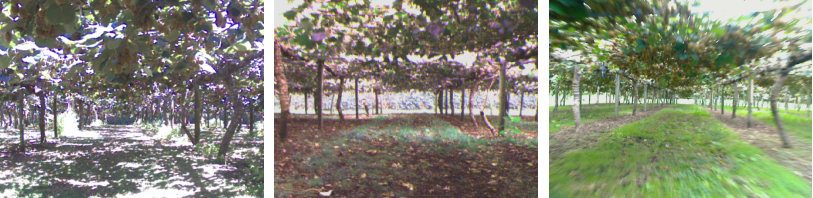
\includegraphics[width=\linewidth]{imgs/camera_comparison/camera_comparison.pdf}
            \caption{
                Example images captured from trialled 2D cameras.
                Basler Dart daA1600-60uc (left), Flir CM3-U3-13S2C-CS (centre), Logitech C920 web-camera (right).
            }
            \label{fig:canopyDataCloud}
        \end{figure}

        Images from the industrial 2D cameras (from Basler and Flir) were deemed suitable for object detection and classification.
        This was verified by processing the data using readily accessible detection algorithms such as convolutional neural networks.
        Both the time-of-flight and 3D stereoscopic camera systems were deemed unsuitable based on the occurrences of data loss.

    \subsubsection{In-orchard Lidar Evaluation}
        Three lidar were evaluated, two single-plane and one multi-layer.
        The two single-plane lidar were the Hokuyo UTM-30LX and a SICK LMS111.
        The multi-layer lidar is a Velodyne VLP-16 which has 16 horizontal \SI{360}{\degree} planes spread over \SI{15}{\degree} vertically.
        Data was collected from each lidar by driving through orchard rows with the sensor placed \SI{0.8}{\meter} above ground level.
        Data was captured both on the presented platform and the smaller robots used to collect camera data.

        \begin{figure}[htb]
            \centering
            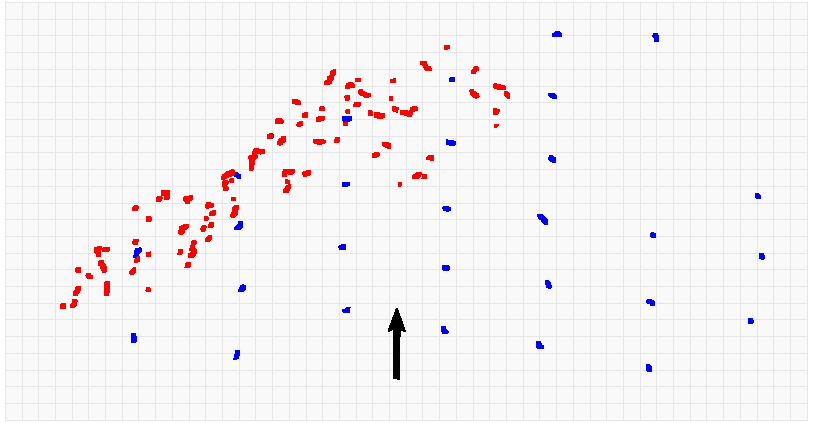
\includegraphics[width=\linewidth]{imgs/canopy_data/canopy_data.pdf}
            \caption{
                Data captured from a single plane lidar showing non-structural points reflected by the canopy (indicated by red markers) and structural points from tree trunks and posts (blue markers).
                The arrow indicates the position and heading of the platform at the time of capture.
            }
            \label{fig:canopyDataCloud}
        \end{figure}

        The intention was to use lidar as a means of detecting structure defining features of the orchard, such as posts, trunks and hedges.
        Detecting these features should allow for row boundary detection and general mapping and localisation.
        However, both single-plane lidar produced clouds of unstructured data amongst the structured features, as shown in Figure~\ref{fig:canopyDataCloud}.
        This was caused by the lidar's scan plane intercepting with the canopy whilst driving over convex terrain.
        Similarly this issue arose on concave terrain where the plane intercepted with the ground, as depicted in Figure~\ref{fig:concaveSlope}.

        \begin{figure}[htb]
            \centering
            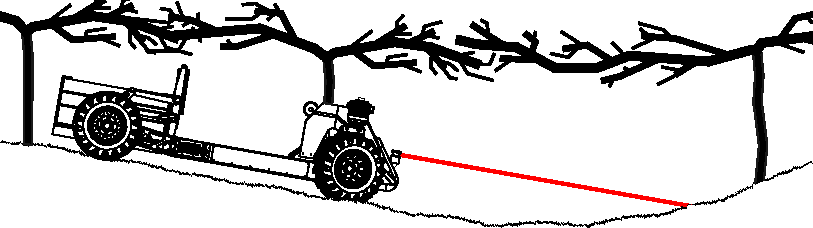
\includegraphics[width=\linewidth]{imgs/concave_slope/concave_slope_v4.pdf}
            \caption{
                On concave slopes the lidar scan plane intercepts with the ground instead of trunks or posts.
                The dashed line shows a horizontal plane coming from the the lidar.
                Dotted lines represent the upper and lower layers taken from the multi-layer lidar.
            }
            \label{fig:concaveSlope}
        \end{figure}

        This issue was reduced by the use of a multi-layer lidar and post-processing.
        Having sixteen layers available meant it was possible to select a scan layer that gives the most useful viewing range.
        Referring again to Figure~\ref{fig:concaveSlope}, that would correspond to the dotted line above the horizontal (dashed) line which intercepts with a row defining feature (a tree trunk).

        It was decided that a multi-layer lidar would be best suited for navigation due to its ability to to see more distant features while driving on undulating ground.
        A single-plane lidar could still be used at short range as an independent channel of processing for redundancy or obstacle detection.

    \subsubsection{In-orchard GNSS Evaluation}
        Two GNSS receivers were evaluated: a Ublox Neo-M8N module and an OmniSTAR 5120VBS with AX0 series antenna.
    	Both were connected to a single board computer (Beaglebone Black) via serial connection.
        The Ublox module was selected for its high sensitivity and internal low-noise amplifier.
        It is capable of receiving GPS, Galileo, GLONASS, and BeiDou GNSS signals concurrently.
        The OmniSTAR receiver was chosen for its external high-gain antenna (34 dB) which claims multi-path rejection.
        It is capable of receiving only GPS signals.

        The testing procedure first involved planning a path through a single row of a kiwifruit orchard and plotting this on a satellite map.
        % Waypoints were placed along the row at the location of posts used to hold the canopy's structure.
        % Relative distances between these waypoints were measured with a tape measure and recorded.
        The receivers were then tested separately over the course of approximately two hours by walking them along the planned path.
        Before testing, each unit was powered up and given \SI{30}{\minute} to initialise in an open area near the kiwifruit orchard.
        During testing, each unit was walked slowly along the predetermined path with stops at each waypoint to provide time for a positional fix.
        The path was approximately \SI{500}{\meter} in length and took approximately \SI{15}{\minute} to complete, including stops at each waypoint.
        Waypoints were spaced at intervals of \SI{5.5}{\meter} along the row.

        \begin{figure}[htb]
            \centering
            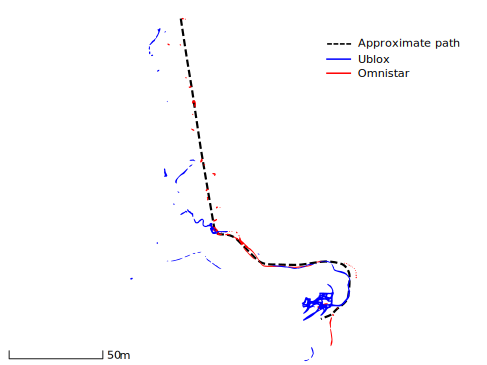
\includegraphics{imgs/gps_path/gps_path.pdf}
            \caption{
                Aerial view of the path taken through the test orchard and the captured GPS data.
                Dashes representing the approximate path are spaced at intervals of \SI{5.5}{\meter}.
            }
            \label{fig:gpsResults}
        \end{figure}

        The path followed, together with coordinates collected from the receivers, are presented in Figure \ref{fig:gpsResults}.
        It should be noted that data has been recorded for the round-trip so represents two passes along the path.
        It was noticed during testing that the signal quality lights on both receivers regularly indicated a loss of signal.

        The Omnistar unit appears to track the approximate path well, but the data is sparse with regular loss of signal after entering the orchard.
    	The Ublox unit collected more data, but was much less accurate.
        It may be possible to use a unit such as the Omnistar, which provided fewer but more accurate readings, as a sanity check for an approximate location within orchards.
        Overall, the units could not be relied on for localisation in this environment.
        These results indicate GNSS receivers with similar performance to those trialled are unsuitable for use in kiwifruit orchards.



% \subsection{Data Collection and Inspection}
 %    The sensors that seemed important to test, based on both the literature survey and the cost-benefit analysis were lidar, cameras and GPS.
    % In addition, time of flight cameras were considered, because they seemed to be a compelling option based on the cost-benefit analysis; especially if some of the less expensive models were found to work well in sunlight.
    % It was also decided that encoders would be tested in favour of using an IMU because the encoders were built into the AMMP motors.
    % Some data was collected from each sensor in order to decide which sensors to prototype algorithms for.


    % \subsection{Sensor Demonstration by Prototype Algorithm}

    %     Basic tests indicated that multi-layer lidar and 2D cameras were best suited for use as primary in-orchard navigation sensors.
    %     Further testing with prototype navigation algorithms ensured that these apparent sensor benefits translated into practical advantages.

    %     The three goals for the navigation system are:
    %     \begin{itemize}
    %         \item object detection and classification,
    %         \item mapping and localisation, and
    %         \item orchard row tracking.
    %     \end{itemize}
    %     To validate that the sensors could perform these functions, three prototype navigation algorithms have been created.

    %     \subsubsection{Object Detection and Classification}

    %         % Object detection and classification was firstly prototyped fully on the camera data.
    %         Based on existing success using convolutional neural networks for image processing tasks \citep{LeCun2015}, a camera based system was chosen for object detection and classification.
    %     	The network architecture chosen was FCN-8s \citep{long2015}.
    %         It is a neural network made of convolutional layers without fully connected layers.
    %         % convolutional layers at the input and fully connected layers at the output.
    %     	FCN-8s performs semantic segmentation, which refers to the per-pixel classification of images.

    %         To train the FCN-8s network, the same image dataset used to assess camera performance earlier was hand labeled.
    %     	Labeling involved drawing object outlines in each image, filling those outlines with colours corresponding to the object's type, and filling any non-labeled areas with black.
    %         Each image was then converted to an indexed colour file format.
    %     	An example of an original image and its corresponding label image is shown as figure \ref{fig:segImgLabelPair}.

    %         \begin{figure}[htb]
    %             \centering
    %             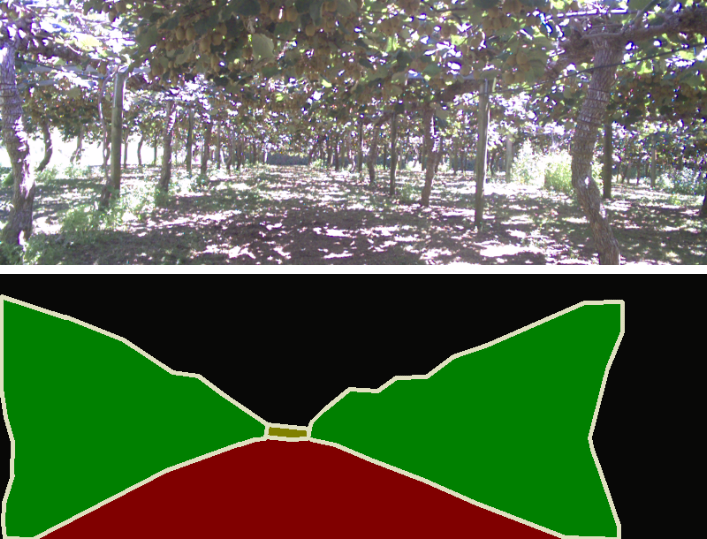
\includegraphics[width=\linewidth]{imgs/photos/segImgLabelPair_trimmed.png}
    %             % \includegraphics[width=\linewidth]{imgs/photos/segImg_sideBySide.png}
    %             \caption{
    %                 An input image (top) and labeled output (bottom) used to train the semantic segmentation network.
    %             }
    %             \label{fig:segImgLabelPair}
    %         \end{figure}

    %         \begin{figure}[htb]
    %             \centering
    %             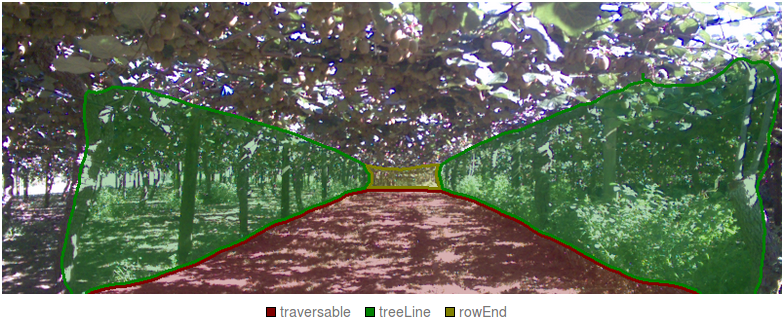
\includegraphics[width=\linewidth]{imgs/photos/semSegRowResults.png}
    %             \caption{
    %                 An example inference result from the trained FCN-8s network.
    %             }
    %             \label{fig:semSegRowResults}
    %         \end{figure}

    %         Initially, individual trees and posts in the kiwifruit orchard were labeled.
    %     	It was later found that labeling the entire tree-line as a single class gave more robust results.
    %     	Objects labeled for this algorithm are:
    %         \begin{enumerate}
    %         \item traversable space (labeled as red),
    %         \item treelines (labeled as green), and
    %         \item the end of the current row (labeled as tan).
    %         \end{enumerate}
    %         Traversable space was defined as the ground area that the platform could drive directly to without collision.
    %         These labeled images were then used to train the FCN-8s network.
    %     	Sample output from the trained network is presented as figure \ref{fig:semSegRowResults}.

    % \subsubsection{Mapping and Localisation}
    %     An existing Simultaneous Localisation And Mapping (SLAM) package was used to test the multi-layer lidar.
    %     The package used was Gmapping \citep{Grisetti2007}, implemented as a ROS package \citep{Gerkey2010}.
    % 	Required input for Gmapping is odometry data and a single plane of lidar data.
    %     Odometry information was provided by the platform's in-built wheel encoders.

    %     \begin{figure}[htb]
    %         \centering
    %         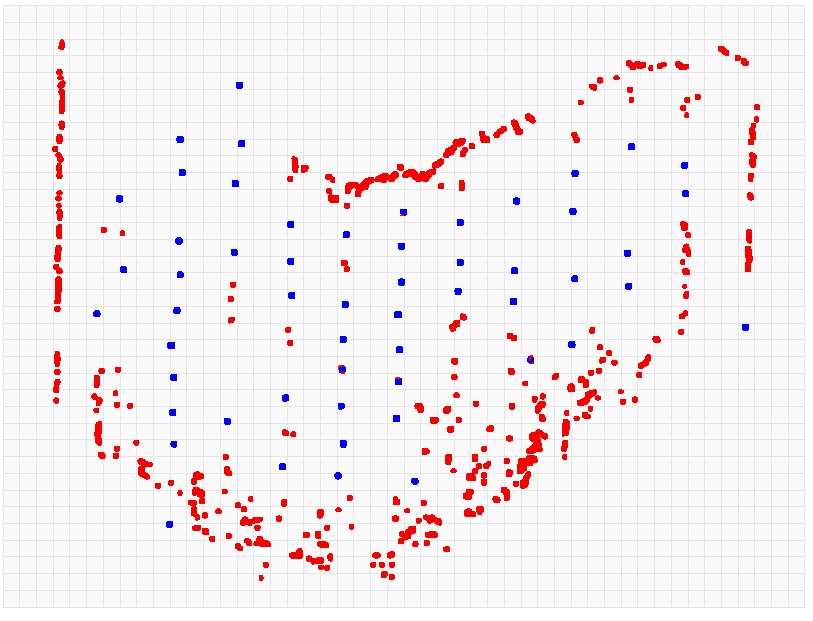
\includegraphics[width=\linewidth]{imgs/single_plane_extraction/single_plane_extraction.pdf}
    %         \caption{
    %             Processing of multi-layer lidar data into a single plane equivalent.
    %             Blue points are those selected by the algorithm for further processing, whereas red points are rejected.
    %         }
    %         \label{fig:singlePlaneExtraction}
    %     \end{figure}

    %     As the multi-layer lidar has 16 scanning layers, a conversion was necessary to produce the single plane of data required by Gmapping.
    %     The simplest conversion from multi-layer data to a single plane would be to select one of the available planes and discard the remaining data.
    %     However, that approach would loose any benefit offered by the multiple scanning layers.
    %     Instead, filtering the multi-layer data into a single plane was done by examining the centre four scan layers at each azimuth.
    %     With this algorithm, if the range difference between all four points at a single angle falls below a certain threshold, the closest point is returned.
    %     Alternatively, if the spread in points is above the threshold, no points are returned.
    %     This eliminates points from sloped or varying surfaces while still returning points from objects with vertical structure.
    %     The effect of this is that the orchard's structural elements remain visible, but ground and canopy information are removed.

    %     \begin{figure}[htb]
    %         \centering
    %         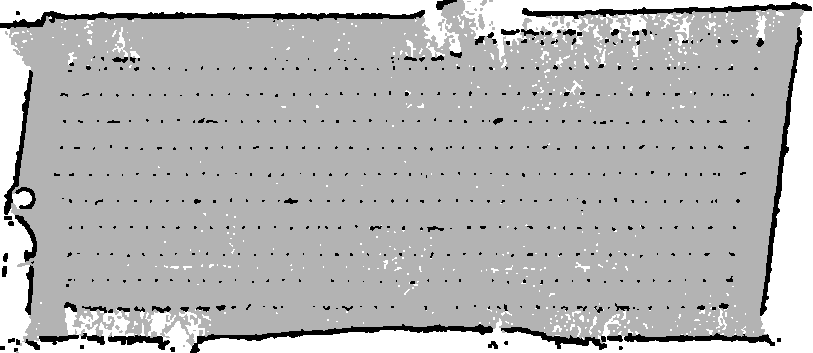
\includegraphics{imgs/gmapmap/gmapmap.pdf}
    %         \caption{
    %             A resulting SLAM based map of a kiwifruit orchard created using Gmapping.
    %             Data for the map was collected by traversing four of the orchard's ten rows.
    %             Odometry information has been taken from wheel encoders and a multi-layer lidar (Velodyle VLP-16).
    %         }
    %         \label{fig:gmapmap}
    %     \end{figure}

    %     The filtered points are then fed into Gmapping as a single plane with data from the platform's wheel encoders.
    %     Figure~\ref{fig:singlePlaneExtraction} shows the method's ability to filter structural elements from data containing significant canopy and ground reflections.
    %     Using this method, a SLAM based map of the orchard was created and is presented as figure \ref{fig:gmapmap}.


    % \subsubsection{Kiwifruit Orchard Row Tracking}
    %     \label{sect:row_tracking}

    %     Our final navigation test required interpreting the orchard's structure for the purpose of path generation.
    %     For this, a row guidance system was developed and tested.
    %     It uses the multi-layer to single-plane data filtering technique discussed previously.
    %     This algorithm also makes use of the platform's on-board wheel encoders.
    %     Details of this algorithm have been published separately \citep{Bell2016}.
    %     The key function of this algorithm is computing the angular offset of the platform from the row's centre-line.

    %     A visualisation of data captured whilst navigating the kiwifruit orchard is presented as figure \ref{fig:lastLidarFrame}.
    %     The method does not perform SLAM, so the visualised data represents only the sensor's current input, i.e., previous sensor data is not considered.
    %     Figure \ref{fig:lastLidarFrame} shows that while the algorithm is not perfect, it does perform reasonably well at identifying orchard structure and generating valid headings.

    %     \begin{figure}[htb]
    %         \centering
    %         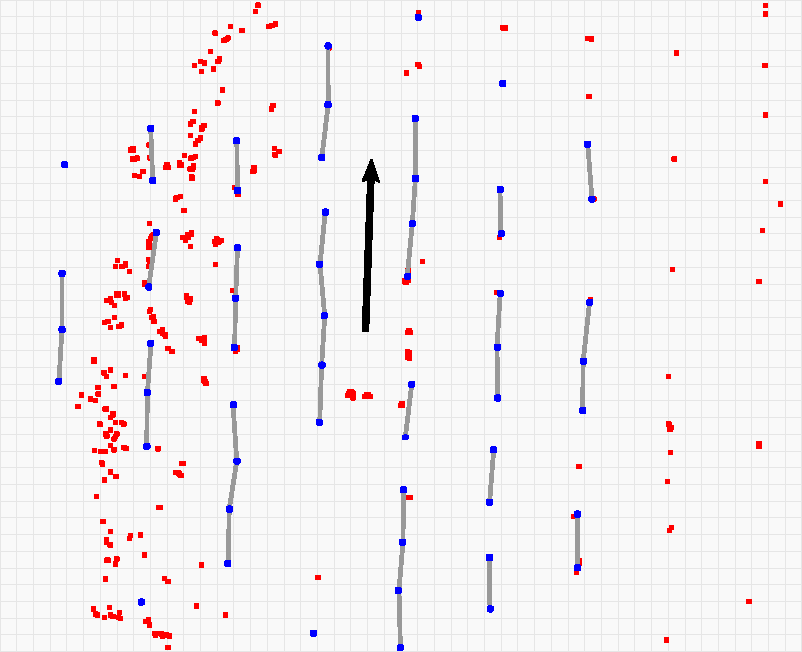
\includegraphics[width=\linewidth]{imgs/row_following/row_following_narrow.pdf}
    %         \caption{
    %             Row detection from multi-plane lidar data.
    %             Red points indicate non-structured data that have been ignored.
    %             Blue points indicate orchard structure data used for row navigation.
    %             Grey lines link orchard structure points by their nearest neighbors (performed algorithmically).
    %             The black arrow represents the centreline of the row current row.
    %         }
    %         \label{fig:lastLidarFrame}
    %     \end{figure}

\section{Autonomous Block Traversal}
\label{sect:autonomous}
    Two separate row following algorithms were developed based on the sensor selection findings, with details of each published separately.
    One method used the multi-layer lidar to detect individual trunks and posts of the pergola style orchard row and follow a centre-line between them \citep{Bell2016}.
    The second method used a single camera combined with a convolutional neural network to segment features in the image such as traversable space, tree-lines, and row-ends \citep{Bell2017}.
    A centreline was then fitted to the areas marked as traversable and used to generate a control vector.

    Both algorithms were developed on smaller, commercially available, test robots while the target platform was under development.
    A laptop (Dell E6410) with integrated graphics processor (Nvidia M5000M) was used on those platforms to process the sensor data and generate drive commands.
    Both approaches produced paths that led to reproducible row following behaviour.
    A method of conducting row-end turns was trialled on the Pioneer 3-AT robot using the lidar based approach.
    However, the robot's drive system lacked the power required to turn into rows on uphill slopes.

    Both approaches were transferred to the target platform once validated on the smaller robots.
    Differences in the geometry between these platforms meant adjustments were needed.
    The small robots both used skid-steer geometries, whereas the target platform uses Ackermann.
    Operationally this has two implications.
    The first is that when turning, the smaller robots pivot along an axis that passes through the mid-point of their chassis.
    On the full-sized platform, that axis instead passes through the centre of the rear wheels.
    Secondly, the full-sized platform must change the angle of its steering wheels before it can begin changing direction, adding a delay.
    A skid-steer geometry only needs to change the relative angular velocities of its wheels.
    These differences are minor when row following as only small changes in angle are required to keep the vehicle on track.
    Alterations were made to account for new pivot axis, but not for actuation delay.

    To determine when the robot is at the end of a row, the multi-layer lidar is used to detect the absence of canopy in a volume above the front and to the sides of the vehicle.
    This method was used to initiate a row-end turn maneuver in the case of both the lidar and camera based approaches.

    \color{red} This is where the row end turn stuff gets added!!!!!!!!!!!!!!! \color{black}

    A row-end turn sees the platform execute a series of maneuvers which have previously been recorded for the specific row and direction of turn.
    Initially, a template maneuver is executed at each row-end and the vehicle is observed while executing the turn.
    Manual adjustments are made to the recorded turn profile based on the vehicle's proximity to obstacles or nearby boundaries during the maneuver.
    Turns are repeated and the profile adjusted until a satisfactory and reproducible turn is established.
    A turn profile can contain any number of steps, with each step being a distance to travel or angle to turn through with a given radius.
    If an object is detected in the vehicle's path during a turn, the steering is adjusted to avoid the object.
    Figure \ref{fig:suzy_turning} shows the platform performing a row-end turn while under autonomous control.

    \begin{figure}[htb]
        \centering
        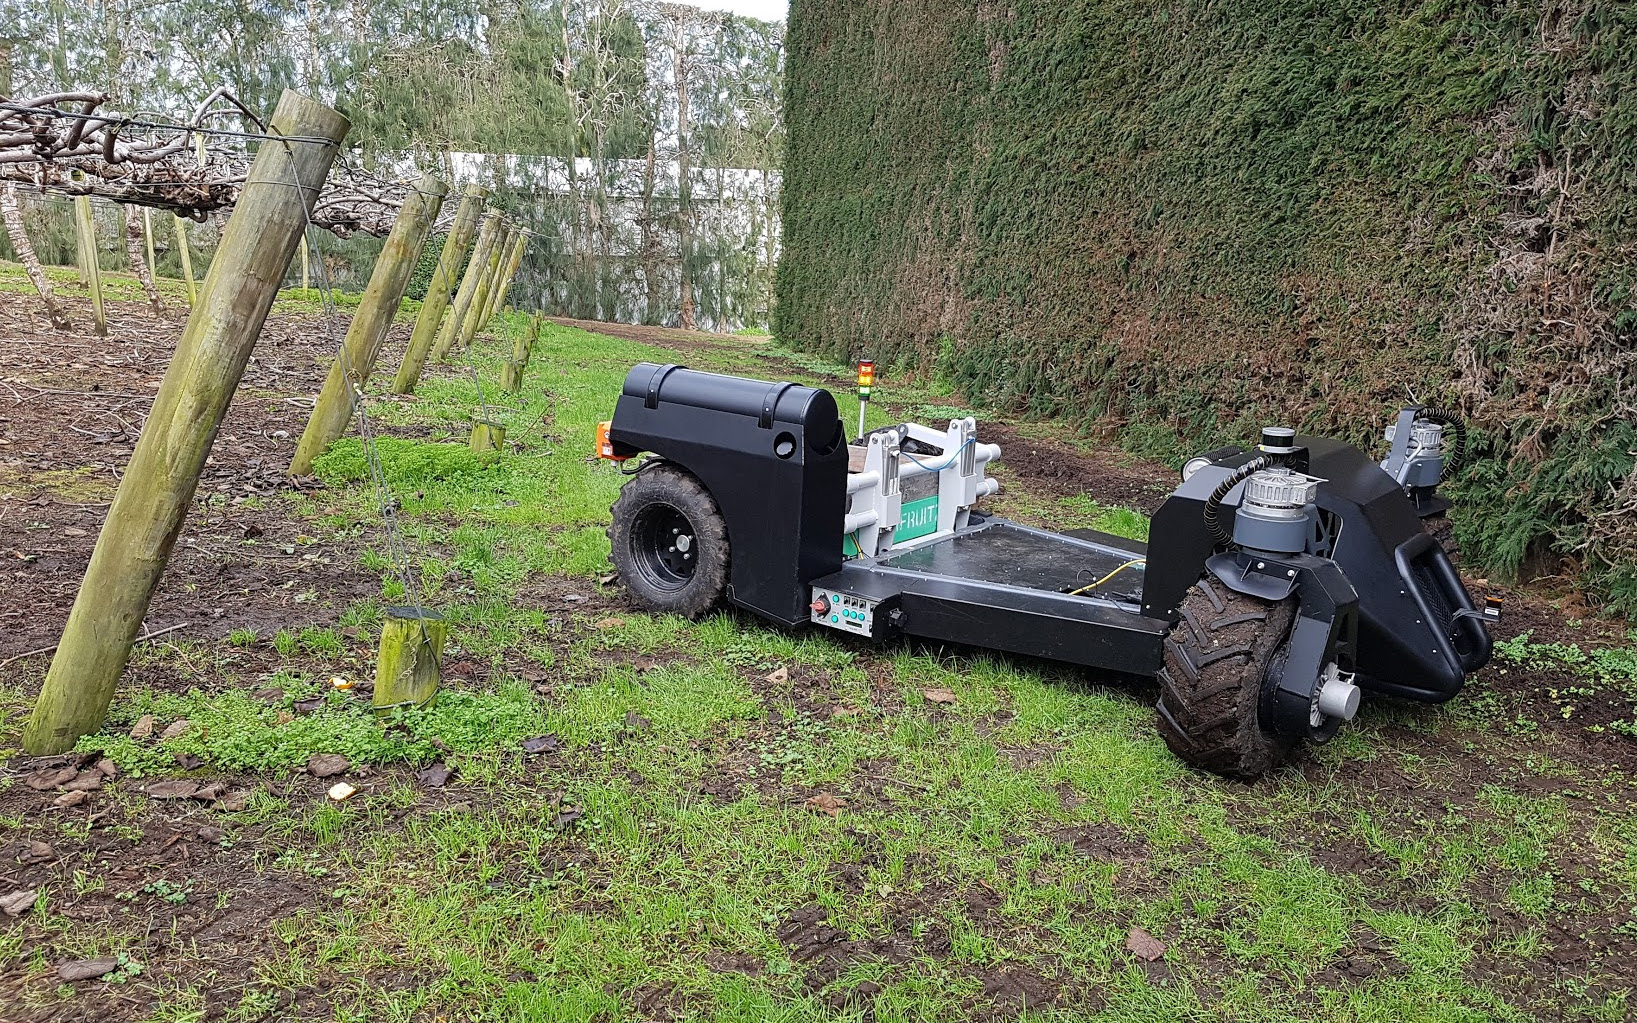
\includegraphics[width=\linewidth]{imgs/photos/suzy_turning.jpg}
        % 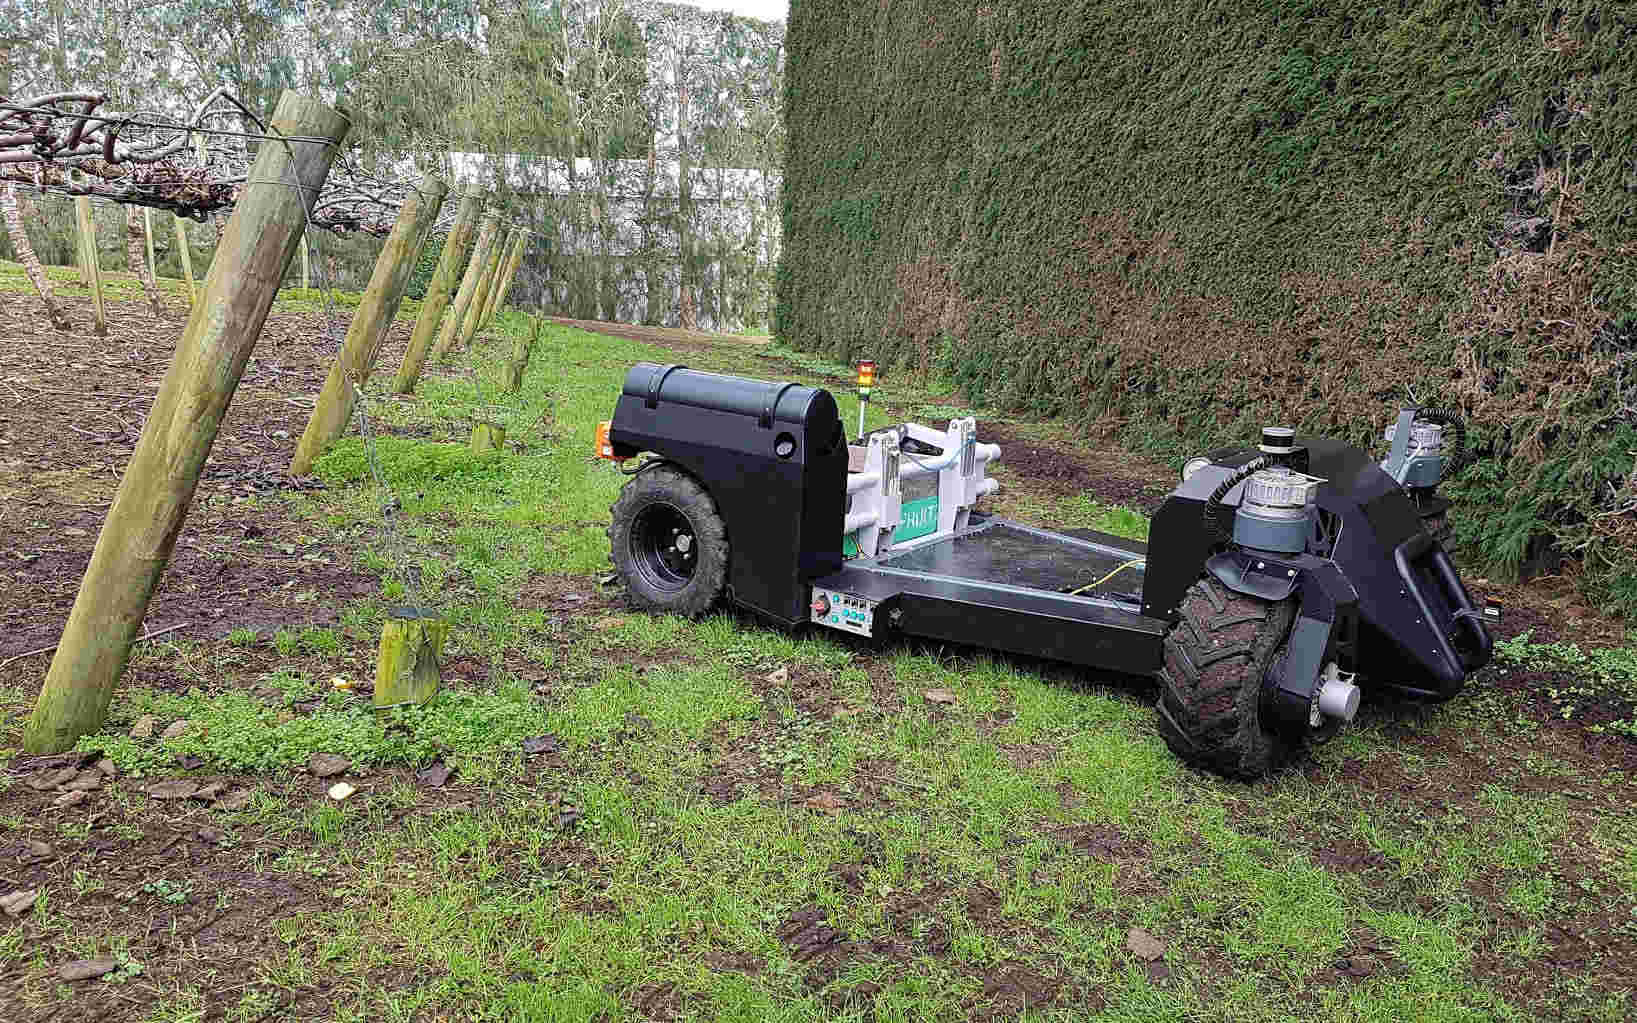
\includegraphics[width=\linewidth]{imgs/photos/suzy_turning_small.jpg}
        \caption{
            The platform performing a row-end turn in the headland area of a kiwifruit orchard while under autonomous control.
        }
        \label{fig:suzy_turning}
    \end{figure}

\section{Testing}
\label{sub:testing}

    % Low-level software to control the platform's drive system was tested in simulation before deployment onto physical hardware.
    % As was the case during development of BoniRob, the open source robot simulation package Gazebo was used.
    % Tests revealed bugs in some of the geometry calculations that were amended before deployment on hardware.

    Structural integrity testing was carried out by strapping a \SI{1100}{\kilo\gram} mass to the vehicle's module area.
    No deflection of the vehicle's chassis structure was evident upon application of the test mass.
    Deflection of approximately \SI{1.5}{\milli\meter} was measured between the front pivot and the wheel supports.

    \begin{figure}[htb]
        \centering
        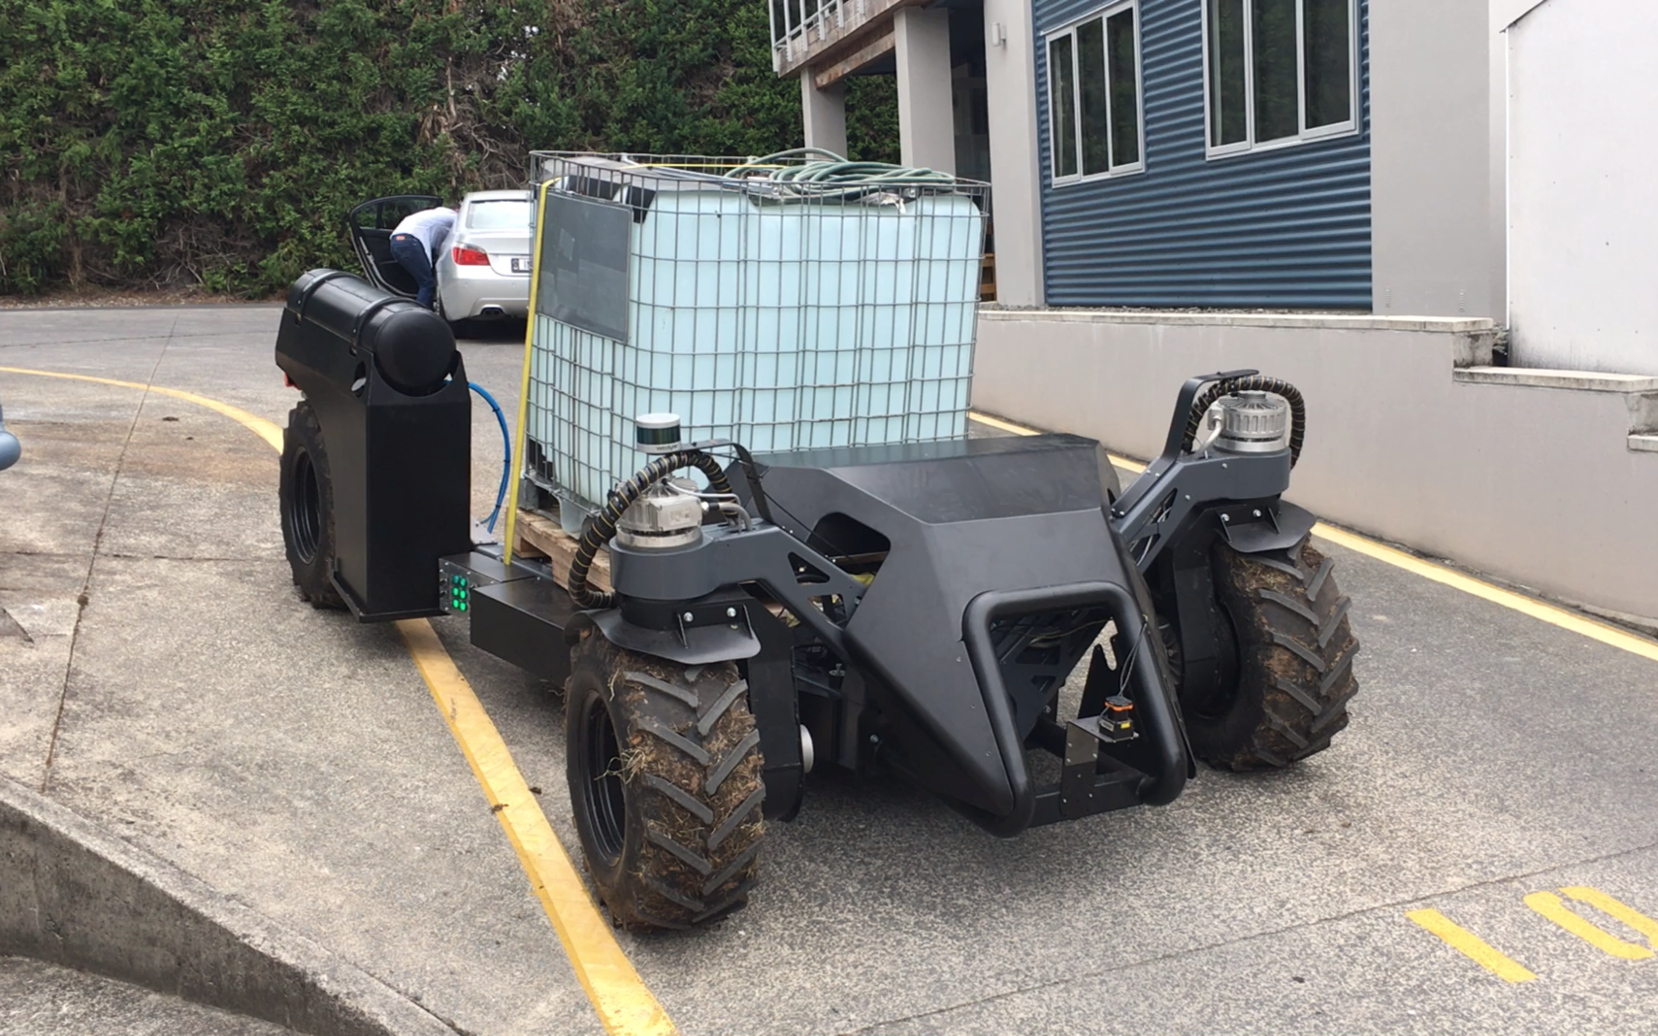
\includegraphics[width=\linewidth]{imgs/photos/stopTesting.jpg}
        % 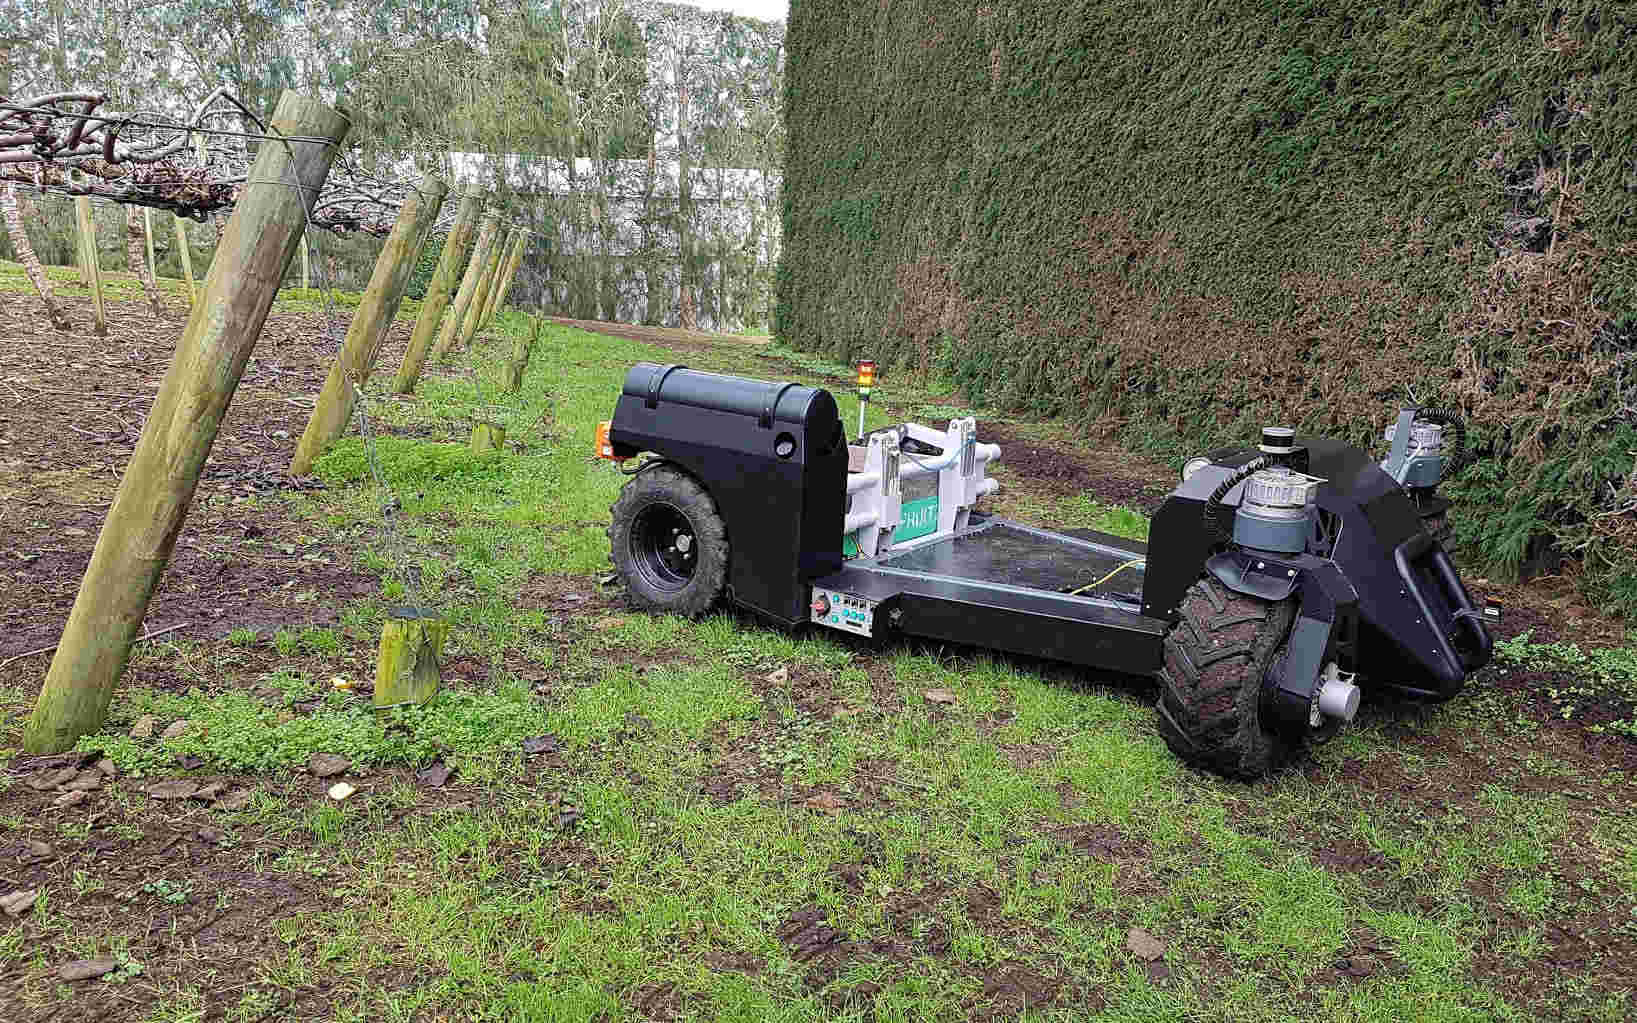
\includegraphics[width=\linewidth]{imgs/photos/suzy_turning_small.jpg}
        \caption{
            Stop testing down a \SI{10}{\degree} slope with a \SI{1100}{\kilo\gram} mass strapped to the module area.
        }
        \label{fig:suzy_testing}
    \end{figure}

    Static steering tests conducted on a dry concrete surface showed no reduction in ability to turn while supporting the test mass.
    Dynamic tests involved three instances of stopping whilst driving down a \SI{10}{\degree} slope at a speed of \SI{10}{\kilo\meter\per\hour}.
    During each test the vehicle came to a complete stop within a distance of \SI{2.4}{\meter}.

    The platform was routinely able to navigate two test blocks, denoted Block A and Block B, from separate orchards using the lidar based navigation approach approach.
    Block A is \SI{1.15}{\kilo\meter} in total traversable length spread over 10 rows.
    Block B is \SI{670}{\meter} in total traversable length spread over 9 rows.
    After tuning of the row end turn maneuvers, the platform navigated Block A consecutively 7 times.
    Figure \ref{fig:block_traversal_bateman} shows the number of interventions per traversal while under tuning in Block A, 18 traversals in total.
    After tuning the row end turns in the second block, this block was navigated 3 times consecutively.
    Figure \ref{fig:block_traversal_newnham} shows the number of interventions per traversal while under tuning in Block B, 9 traversals in total.
    This equates to a total of \SI{10}{\kilo\meter} of successfully navigated orchard rows.


    \begin{figure}[htb]
        \centering
        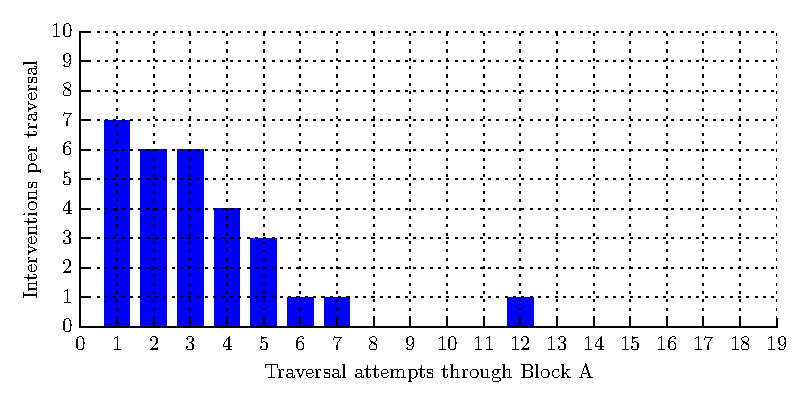
\includegraphics{imgs/tuning_graphs/bateman.pdf}
        \caption{
            Number of interventions during tuning of row-end turns throughout Block A.
        }
        \label{fig:block_traversal_bateman}
    \end{figure}

    \begin{figure}[htb]
        \centering
        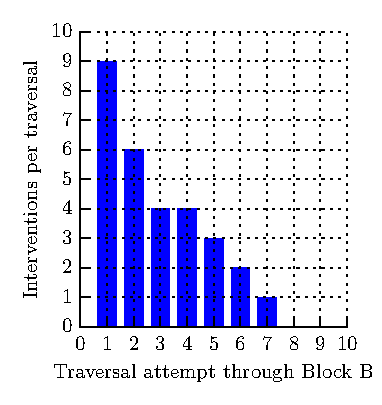
\includegraphics{imgs/tuning_graphs/newnham.pdf}
        \caption{
            Number of interventions during tuning of row-end turns throughout Block B.
        }
        \label{fig:block_traversal_newnham}
    \end{figure}


    % Any time the vehicle had to be taken out of autonomous control during a block traversal are counted as failed attempt.
    The key weakness of the current navigation system is the need to tune the row end turns manually for each site.
    The tuning required for the first orchard block amounted to six traversals of the entire block.
    For the second block, five complete traversals were required for tuning.
    This creates a significant resource overhead for deployment to any new sites.
    If the row end turns are not sufficiently tuned, two failure cases may occur.
    The most common case is that the vehicle turns through a row end too tightly or not tightly enough and the object avoidance system is not sufficiently responsive to avoid a collision.
    There were nine traversals where an operator intervened during row end turning.
    Seven of these were due to an imminent collision with a post during a row end turn.
    The remaining failures during row end turning were due to the platform trying to recommence row following before facing the new target row.
    In this case the most feasible path for row following was detected through the headland area, instead of the target row.

    % Simulation of the software responsible the Ackermann steering geometry revealed software bugs.
    % These bugs were
    % The open source robotics simulation package Gazebo was used to simulate the vehicle, which allowed driving it using a game controller.


\section{Discussion}
\label{sect:discussion}

    The reported platform achieves the requirements outlined during the introduction and has proved its usefulness during two pollination and harvesting seasons.
    However, during these operations the vehicle was primarily operated under manual control.
    This was due to the need to control the vehicle outside of its autonomous operating behaviour.
    In most cases it was driven as close as possible to a row's edge on two passes through each row.
    This was necessary to give mounted modules access to the full canopy area whilst performing their tasks.
    The need to drive close to row boundaries was unexpected as the modules were expected to require only a single pass per row.

    The results from testing of navigation algorithms indicate that the multi-layer lidar and wheel encoder feedback are enough row following tasks.
    This combination alone has proven successful for autonomous driving in two kiwifruit orchards.
    A combination of 2D cameras and neural networks was suitable for object detection and classification, and for generating headings for row following.
    The two approaches for row following proved reliable, however the method for turning between rows calls for further work.
    Row end turning was a manual process that involved observing an autonomously driven turn and manually adjusting the length or radius of the turn's segments.
    Future work will focus on enabling the system to plan row-end turns based on sensor data, without a manually created map.

    During installation and testing of the platform's electrical system, the \SI{96}{\volt} battery pack introduced a significant electrical hazard.
    While essential for safety, risk mitigation procedures added complexities and delays that could have been avoided by selecting a lower pack voltage.
    The authors suggest a pack voltage of \SI{48}{\volt} as a safer alternative during vehicle development as it bears a reduced risk of injury from electric shock.
    Inputs of \SI{48}{\volt} are supported across a wider range of motors, motor controllers, and power converters, but cabling requirements are increased.
    The benefit of using a lower gauge of cable has not outweighed the extra safety procedures required.

    The series-hybrid configuration allows the vehicle to drive and provide power to subsystems without running the petrol engine.
    This is useful in testing scenarios, where people are in close proximity to the vehicle, as it eliminates exhaust fumes and reduces noise and vibration.
    However, robotic modules and the bin lifting mechanism require pneumatic air pressure to operate.
    As the air compressor is belt driven from the petrol engine, it is necessary to frequently run the engine to provide air to these systems.
    An electric air compressor would allow the system to run unassisted by the petrol engine for much longer periods.
    The authors suggest that efficiency losses from frequently running the engine to maintain pneumatic pressure outweigh conversion losses associated with running an electric air compressor.

    The use of more general purpose robots to test navigation algorithms enabled the navigation system to be developed in parallel with the physical hardware.
    Their smaller size eliminated the risk of serious injury and led to a speed up in development and test cycles.
    It also meant that navigation testing could continue while the platform was engaged in other activities.

    Deflection observed through the steering mechanism while the vehicle was loaded with a \SI{1100}{\kilo\gram} mass indicates rigidity issues in this area.
    While this did not affect the ability of the vehicle to accelerate or turn during testing, subsequent stress related issues have arisen in this area.

    Simulation of the robot hardware proved useful for finding software issues before implementation on hardware.
    Most of the time spent developing the simulation went into the creation of a geometric model of the platform.
    This model has also proved useful for visualising the state of the vehicle, using Rviz, in real-time or when replaying recorded sensor data.
    For instance, it is possible to display the angle of the front steering wheels based on encoder feedback while the platform is being driven.
    It is also possible to place a lidar in the model and have the point-cloud data displayed in the vehicle's coordinate frame.



\section{Conclusion}
    This work presented a platform designed specifically for autonomous driving through pergola style kiwifruit orchards.
    The platform is capable of carrying modules with twice the mass of than those previously reported in the literature.
    Sensors suitable for autonomous navigation have been selected, trialled, and demonstrated as being useful as a means of navigating in this environment.
    Tests suggest either multi-layer lidar or a combination of 2D-camera and neural network based processing are sensible choices as primary navigation sensors.
    These results echo those previously reported when navigating in orchard environments.
    Using a map of manually adjusted row end turns the platform has navigated over \SI{10}{\kilo\meter} of orchard blocks without intervention.
    Further work will focus on improving the the mechanism used to trigger the commencement of a row end turn.
    During development, a \SI{48}{\volt} battery pack was identified as being ideal for development vehicles of this size due to safety and component availability.
    The use of smaller, commercially available, robots were valuable as a means to develop navigation software before deployment on full scale platforms.

\section*{Acknowledgements}
This research was supported by the New Zealand Ministry for Business, Innovation and Employment (MBIE) on contract UOAX1414.
The authors acknowledge contributions from Phillip Ross, Gordon Neshausen, Josh Barnett, and Erin Simms who were involved with the design and fabrication of the platform.


%% The Appendices part is started with the command \appendix;
%% appendix sections are then done as normal sections
%% \appendix

%% \section{}
%% \label{}

%% References
%%
%% Following citation commands can be used in the body text:
%%
%%  \citet{key}  ==>>  Jones et al. (1990)
%%  \citep{key}  ==>>  (Jones et al., 1990)
%%
%% Multiple citations as normal:
%% \citep{key1,key2}         ==>> (Jones et al., 1990; Smith, 1989)
%%                            or  (Jones et al., 1990, 1991)
%%                            or  (Jones et al., 1990a,b)
%% \cite{key} is the equivalent of \citet{key} in author-year mode
%%
%% Full author lists may be forced with \citet* or \citep*, e.g.
%%   \citep*{key}            ==>> (Jones, Baker, and Williams, 1990)
%%
%% Optional notes as:
%%   \citep[chap. 2]{key}    ==>> (Jones et al., 1990, chap. 2)
%%   \citep[e.g.,][]{key}    ==>> (e.g., Jones et al., 1990)
%%   \citep[see][pg. 34]{key}==>> (see Jones et al., 1990, pg. 34)
%%  (Note: in standard LaTeX, only one note is allowed, after the ref.
%%   Here, one note is like the standard, two make pre- and post-notes.)
%%
%%   \citealt{key}          ==>> Jones et al. 1990
%%   \citealt*{key}         ==>> Jones, Baker, and Williams 1990
%%   \citealp{key}          ==>> Jones et al., 1990
%%   \citealp*{key}         ==>> Jones, Baker, and Williams, 1990
%%
%% Additional citation possibilities
%%   \citeauthor{key}       ==>> Jones et al.
%%   \citeauthor*{key}      ==>> Jones, Baker, and Williams
%%   \citeyear{key}         ==>> 1990
%%   \citeyearpar{key}      ==>> (1990)
%%   \citetext{priv. comm.} ==>> (priv. comm.)
%%   \citenum{key}          ==>> 11 [non-superscripted]
%% Note: full author lists depends on whether the bib style supports them;
%%       if not, the abbreviated list is printed even when full requested.
%%
%% For names like della Robbia at the start of a sentence, use
%%   \Citet{dRob98}         ==>> Della Robbia (1998)
%%   \Citep{dRob98}         ==>> (Della Robbia, 1998)
%%   \Citeauthor{dRob98}    ==>> Della Robbia


%% References with bibTeX database:

\bibliographystyle{model5-names}
\bibliography{bibliography_jamie,bibliography_mark}


%% Authors are advised to submit their bibtex database files. They are
%% requested to list a bibtex style file in the manuscript if they do
%% not want to use model5-names.bst.

%% References without bibTeX database:

% \begin{thebibliography}{00}

%% \bibitem must have one of the following forms:
%%   \bibitem[Jones et al.(1990)]{key}...
%%   \bibitem[Jones et al.(1990)Jones, Baker, and Williams]{key}...
%%   \bibitem[Jones et al., 1990]{key}...
%%   \bibitem[\protect\citeauthoryear{Jones, Baker, and Williams}{Jones
%%       et al.}{1990}]{key}...
%%   \bibitem[\protect\citeauthoryear{Jones et al.}{1990}]{key}...
%%   \bibitem[\protect\astroncite{Jones et al.}{1990}]{key}...
%%   \bibitem[\protect\citename{Jones et al., }1990]{key}...
%%   \harvarditem[Jones et al.]{Jones, Baker, and Williams}{1990}{key}...
%%

% \bibitem[ ()]{}

% \end{thebibliography}

\end{document}

%%
%% End of file `elsarticle-template-5-harv.tex'.
